%% This is an example first chapter.  You should put chapter/appendix that you
%% write into a separate file, and add a line \include{yourfilename} to
%% main.tex, where `yourfilename.tex' is the name of the chapter/appendix file.
%% You can process specific files by typing their names in at the 
%% \files=
%% prompt when you run the file main.tex through LaTeX.
\chapter{DressCode}\label{sec:DressCode}

\begin{center}
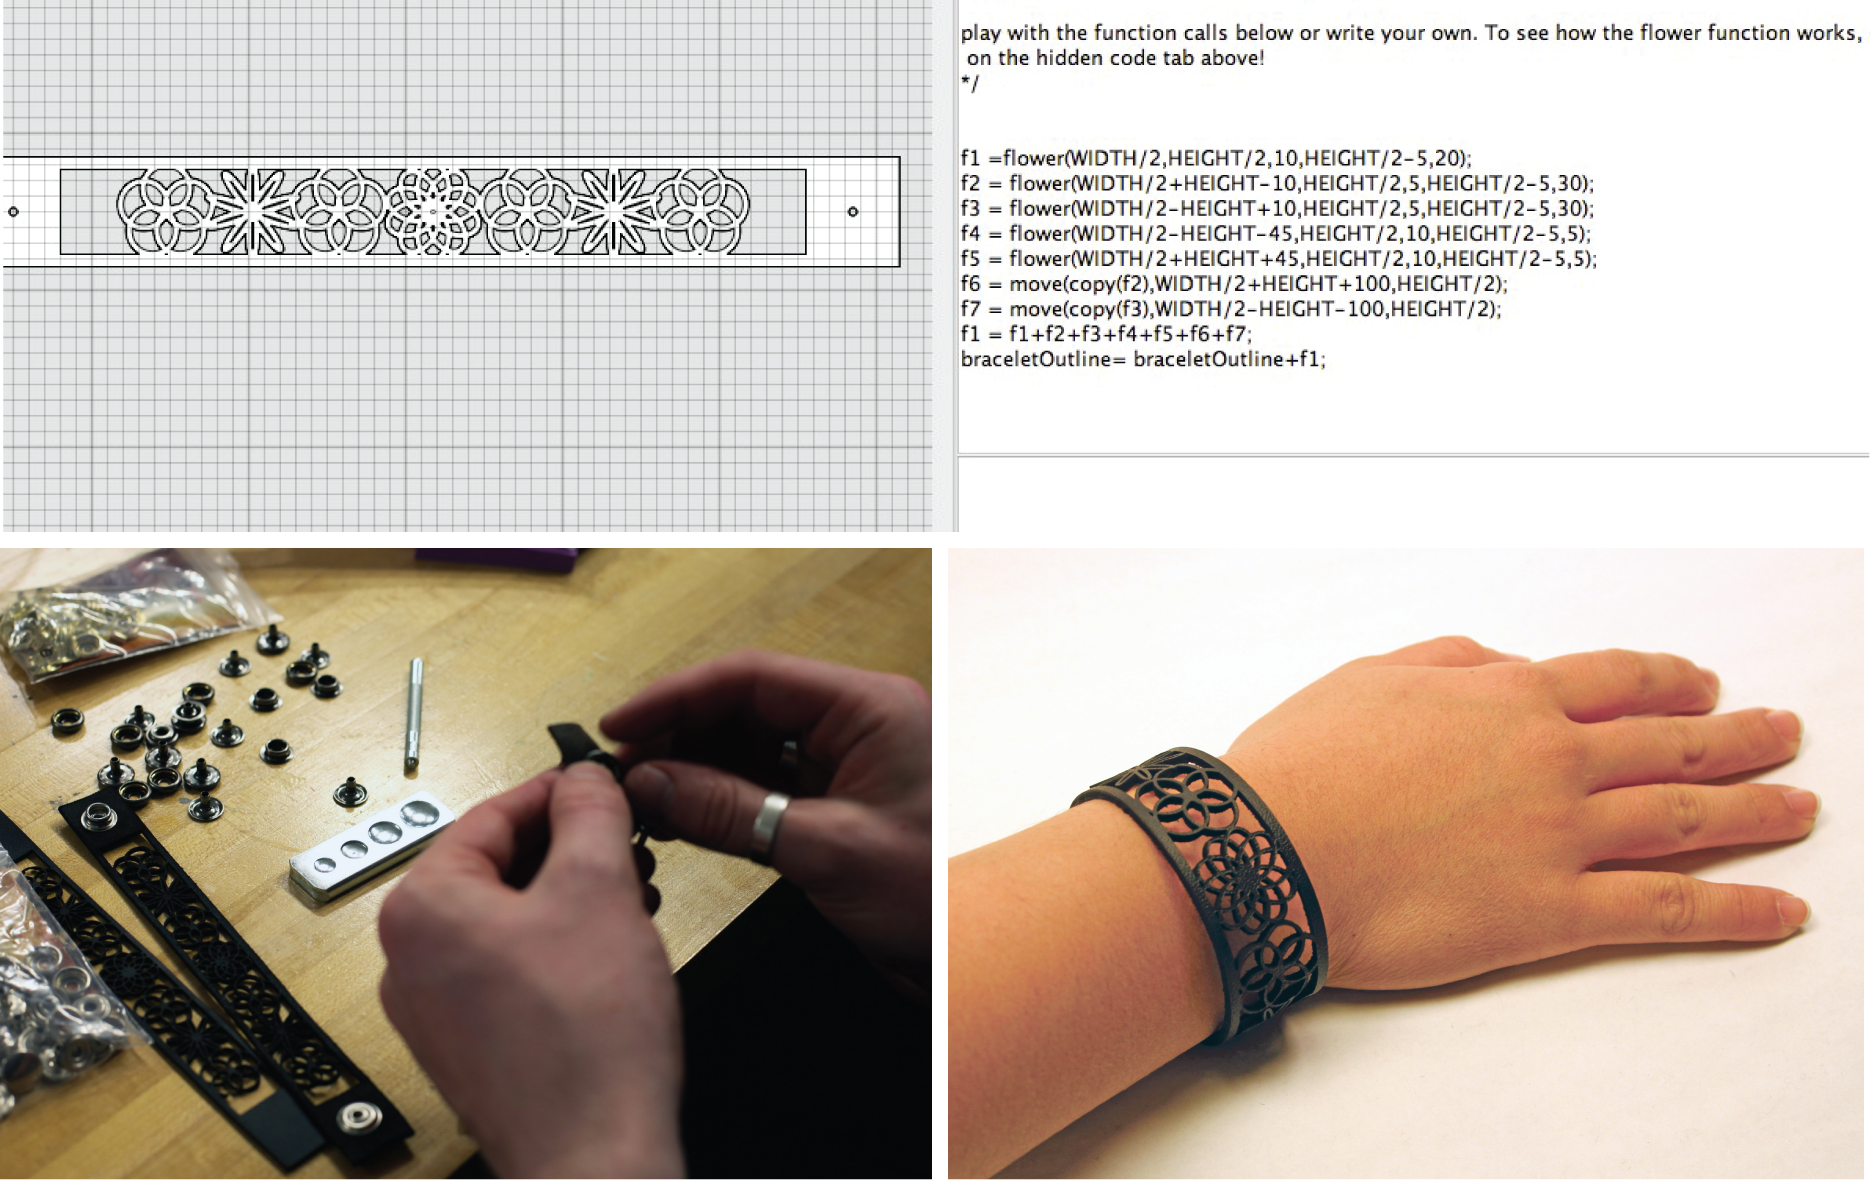
\includegraphics[width=6.5in]{images/dressCode_main.png}
\end{center}


The preliminary work of Codeable Objects and Soft Objects clearly demonstrated that algorithmic craft offers a compelling opportunity for personal, creative expression through programming. My goal following these first two tools was to address several of their primary limitations in an effort to better engage novice programers in the computational design aspects of algorithmic craft. DressCode is a stand-alone programing environment and design tool created to support new programmers in open, independent algorithmic craft. To evaluate Dress Code, I conducted two separate day-long workshops, one with experienced programmers and designers, and one for young people who were new to programming. I also worked with FUSE, an out of school STEAM exploration program to develop a set of online activities using DressCode, which are currently in the preliminary stages of evaluation.	 

\section{Design principles}
Based on the success of the prior fashion workshop, and my continued interest in exploring applications that appeal to women and girls, I decided to focus on computational fashion design and the fabrication of wearable artifacts in the development of DressCode. After reflecting on the potential limitations of this focus however, I decided to develop DressCode as a more open-ended computational design tool that could support the creation of a variety of artifacts, rather than just fashion. To preserve the emphasis on fashion, the majority of the example projects and artifacts I created with DressCode for this thesis were fashion-oriented. The workshops I conducted, as well as the curriculum I helped develop also had an emphasis on fashion or wearable artifacts.

By building my own software, I sought to improve on the preliminary programming libraries in three key areas. First, DressCode contains its own programing language. The DressCode language has a simplified syntax and contains a limited set of textual programming methods, allowing people with little-to-no prior programming experience to working with the language quickly and effectively. Second, the DressCode environment is designed to equally prioritize textual programing and visual design and manipulation. To that end, the software has a two-panel development environment that displays a graphic two-dimensional (2-D) rendering of the user's current design in the first panel, and their code in the second. As a user makes changes to their code, the effects on the design are rendered in the graphic panel. Finally, DressCode contains functionality that is specific to digital fabrication and algorithmic craft. The tool allows for a variety of methods to translate one's design to a tool-paths for fabrication machines. In addition, the API contains programing methods that support the creation of forms and patterns that are suitable for fabrication, with minimal effort on the part of the user.  The goal of designing a software 2-panel programing and design environment, with a specialized programing language and immediate support for digital fabrication was to assist non-programmers in independently making design decisions with programing. In short, I wanted to make it as easy as possible for people to decide on their own desired style or aesthetic, and then realize it by writing their own code. The following section describes the features of the DressCode software in greater detail.

\todo{put in rationale for why dress code is textual rather than visual programing language}

\section{Tool description}
DressCode is a programing and graphical design environment that enables the creation of 2D designs for 2-axis fabrication machines. DressCode is composed both of the application itself, and a custom programing language designed to correspond with the application.

\subsection{Interface Design}
 \begin{center}
\begin{figure}[h!]
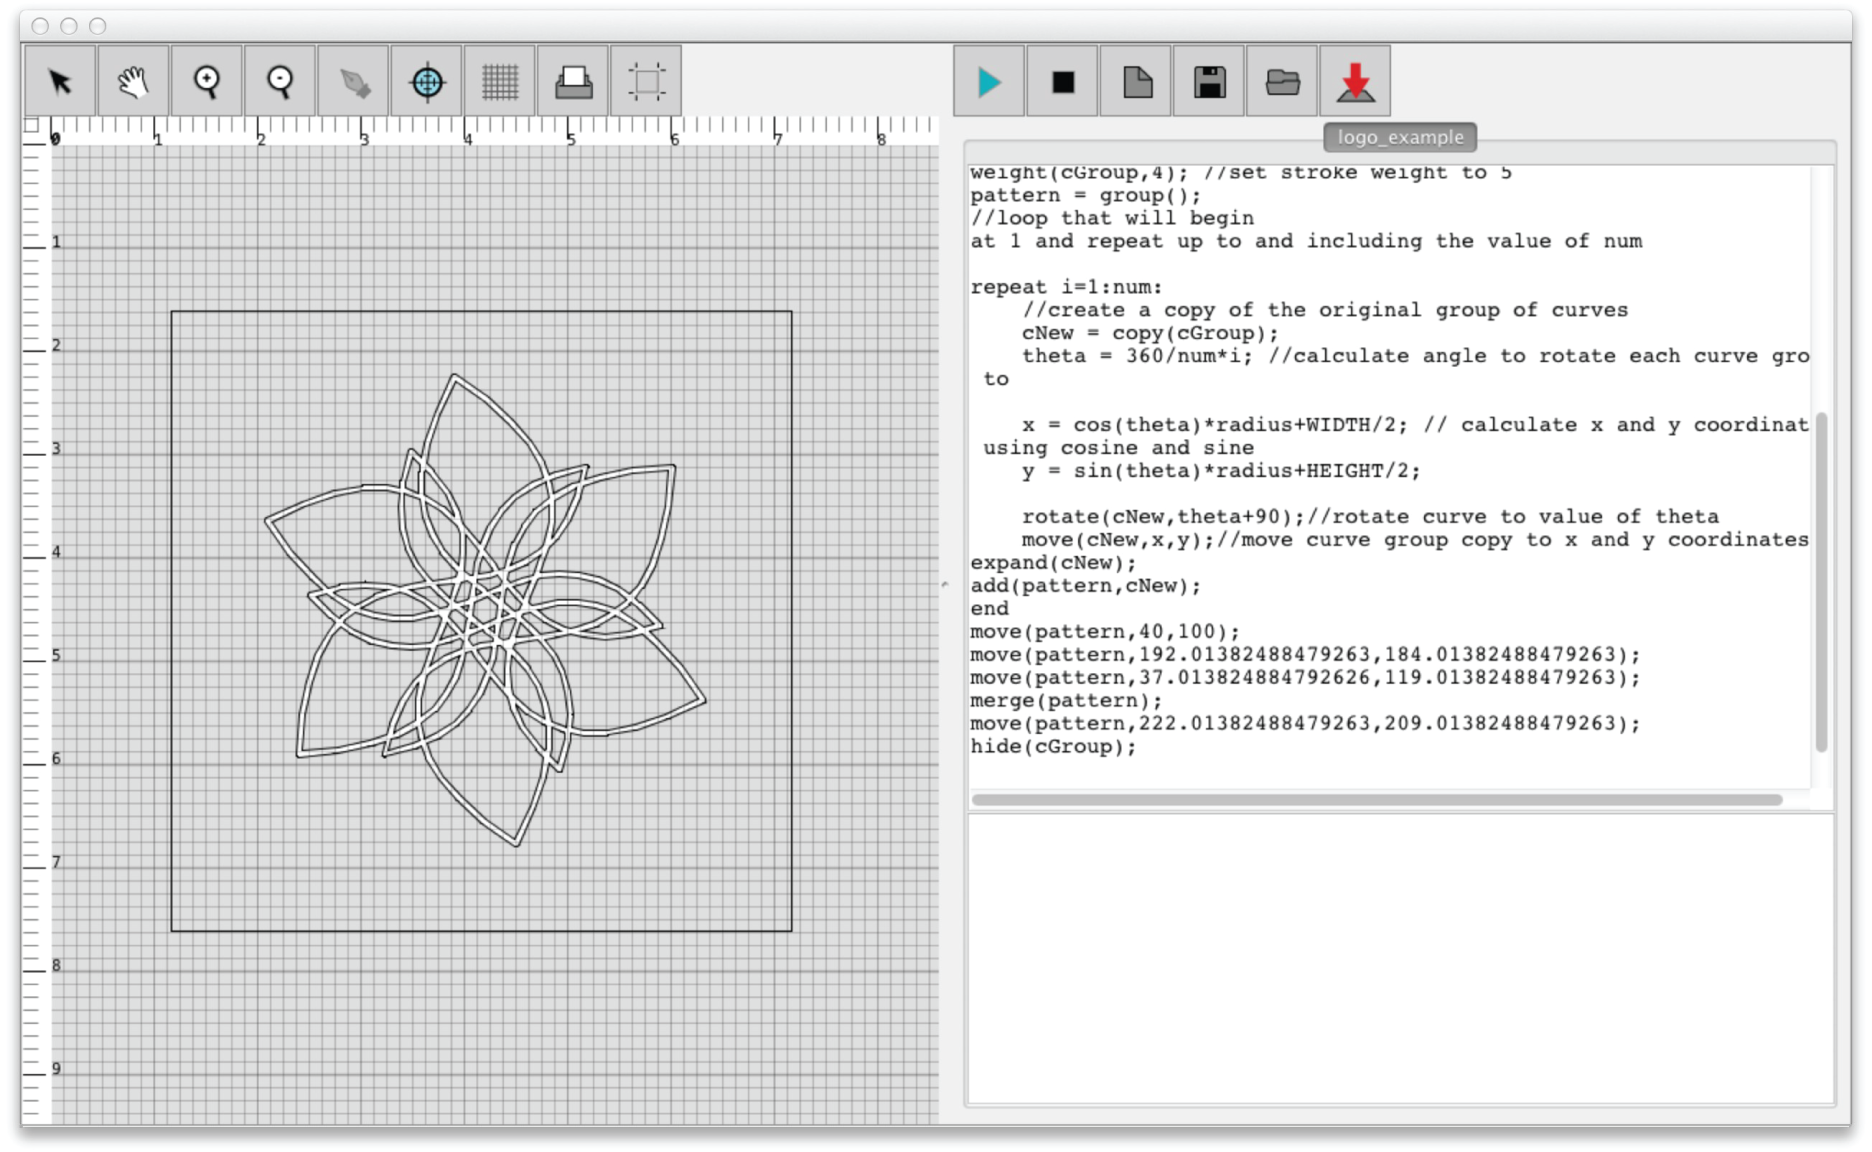
\includegraphics[width=6.5in]{images/dress_code_interface.png}
\caption{The DressCode interface}
\label{fig:dress_code_interface}
\end{figure}
\end{center}

The interface of DressCode is divided into two sections, a design panel and a coding panel. The divider between the two panels can be resized as needed. The coding panel contains a primary window for entering text, an output console for print output and error reporting and a row of buttons on the top. When the play button is pressed, the program in the code window is run and the resulting design is displayed in the design panel. The first version of DressCode ran the code each time the enter key was pressed or a new statement was completed, however we received many requests from our initial user tests for manual control of the run process. The stop button attempts to terminate programs that are taking too long to run.The following three buttons allow for the creation of new programs and the saving and opening of existing programs. The final button opens a dialog that enables the user to select an Scalable Vector Graphics (SVG) file to import into their script (the rationale for this is described in \ref{par:shape_transformation} section below.)

The design panel is primarily composed of the drawing canvas. The drawing canvas has a set of rulers and a grid, along with a black rectangle in the center which serves as the drawing board. The drawing board defines a reference for the coordinate system of the canvas, with the upper left hand corner corresponding to (0,0) in cartesian coordinates. Designs can be drawn on any part of the canvas, including outside the drawing board, however the exported designs file-dimensions will always correspond to the size of the drawing board. The right-most button in the design panel allows for the specification of the units of the project, and the resizing of the drawing board. The print button opens a dialog that allows the user to export their current design in a vector format. I experimented with various vector file formats including DXF, SVG and PDF, however for the time being, I settled on PDFs as they were compatible with the specific fabrication machines I intended to use in my workshops. 

The grid button allows the user to toggle between a grid in the units that correspond to the current units of the project (either millimeters or inches), pixels, or no grid. The target button allows the user to graphically select a set of coordinates and have them appear in the programming window as text, and can be used like an eyedropper for pixel coordinates. The plus and minus magnifying glasses and the hand tool are used to pan and zoom in and out of the screen.  Lastly, the arrow tool allows for design elements to be graphically selected and manipulated. After a design element is moved with the arrow tool, with the corresponding code for the move appears in the programing window. 

\subsection{Programing Language}
The DressCode programing language is interpreted with semantic functionality that is simulated through a Java-based library.  We relied on the ANTLR framework to generate the necessary lexing and parsing methods for the language, and developed the semantic functionality using java and the java openGL (JOGL). When a program is run in DressCode, the raw script is first tokenized and then parsed to generate an abstract syntax tree (AST). During this phase, all user-generated function definitions are stored in memory. If any parsing errors are encountered, they are output to the console as "compiler errors". Assuming the parse is successful, DressCode then walks the resultant AST and attempts to execute the semantic functionality of the program (figure:\ref{fig:interpreter_structure}.) After being executed, the resultant design is rendered on the display panel. Any runtime errors are displayed in the output console. For most programs, this process is instantaneous, however some programs with complex operations require several seconds to be executed. 
  \begin{center}
\begin{figure}[h!]
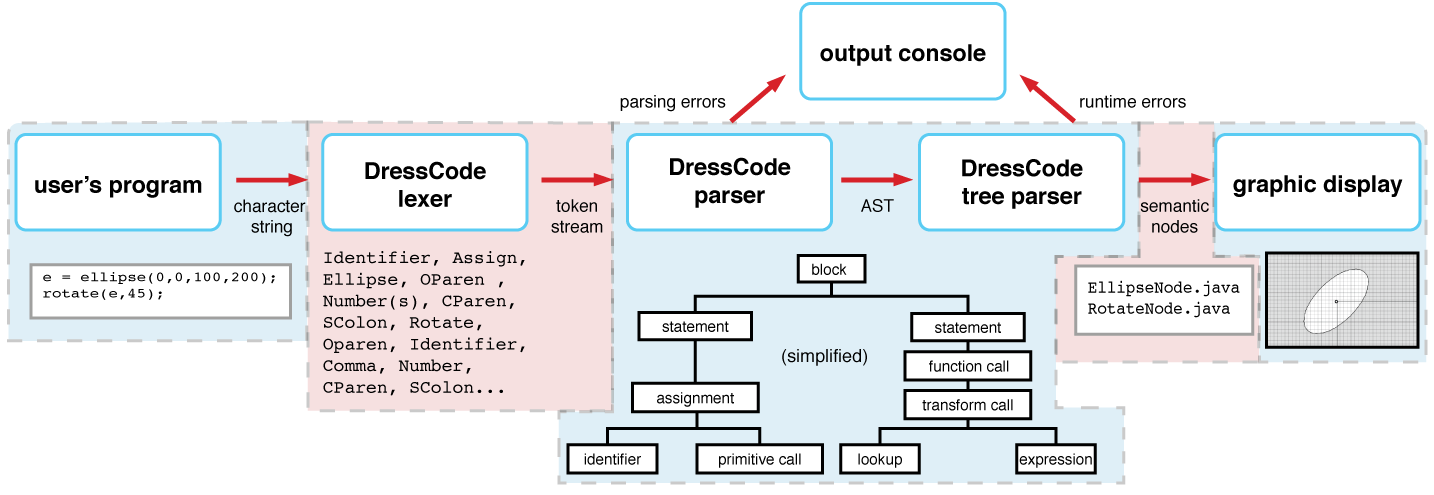
\includegraphics[width=6.5in]{images/interpreter_structure_horz.png}
\caption{Interpreter structure}
\label{fig:interpreter_structure}
\end{figure}
\end{center}
The language is imperative in nature, with statements being executed in the order in which they are read. The exception to this is user defined functions, which may be defined at any point in the program, and called before they are defined. Each statement in DressCode must be terminated by a semicolon. I spent some time experimenting with terminating statements with newlines, similar to whitespace sensitive languages like Python, as I thought this might be more conducive to novice use. Unfortunately, the implementation of selective whitespace recognition is a challenging task to define in a grammar, so while we were able to develop a version of DressCode that recognized statements terminated by a line break, it would have taken significant time to develop this functionality to a level of robustness appropriate for user testing. For the short term, we have opted for a syntax requiring semicolons, however we plan to continue to explore newline statement termination in the future. 

\subsubsection{Language Structure}
Here, I define some of the primary elements of the DressCode syntax and drawing API, and the rationale for their structure. A more thorough language reference is available on the DressCode wiki\cite{DressCodeWiki}.

 DressCode supports number, string, boolean, and drawable datatypes (figure \ref{fig:basic_datatypes}.) The first four of these types are relatively standard in comparison to conventional programing languages. Numbers include integers and floating point values. Strings include any sequence of characters enclosed in double quotations. Booleans have two possible values: true, and false. Drawables are a special type, discussed in detail in the API description below. DressCode also contains a list data structure, which can store multiple kinds of datatypes.
\begin{center}
%\begin{figure}
\begin{lstlisting}
myString = "hello";  //string
myNum = 10.4;  //number
numbermyBool = true;  //boolean
myList = [10,11,false,"world"];  //list with multiple data types
println(myList[3]); //prints world
\end{lstlisting}
%\caption{basic datatypes}
%\label{fig:basic_datatypes}
%\end{figure}
\end{center}

Variable identifiers in DressCode must begin with a letter which followed by 0 or more letters or digits. Variables can be initialized through assignment, or declared and assigned later in the program. All assignment in DressCode is dynamically typed, and variables can be assigned to datatypes that differ from their original assignment at any point. %(figure \ref{fig:variable_assignment}.)

\begin{center}
%\begin{figure}
\begin{lstlisting}
s1 = "hello";
s2 = "world";
s3; //variable without initial assignment

s3 = s1+" "+s2; 
println(s3); //prints hello world

n1 = 2;
n2 = 2.5;
println(n1+n2*10); // returns 27.0
\end{lstlisting}
%\caption{variable assignment.}
%\label{fig:variable_assignment}
%\end{figure}
\end{center}

The  language also contains support for basic expressions, as well as block statements, including conditionals, loops and user-defined functions. For mathematical expressions, standard order of operations is maintained, unless parentheses are introduced. All block statements are signified by a keyword followed by a colon, and terminated with the end keyword which is not followed by a semicolon.Conditionals are defined with the if keyword, and may an optional else clause and  zero or more else if clauses. %(figure: \ref{fig:conditionals}.)

\begin{center}
%\begin{figure}
\begin{lstlisting}
//if statement 
if 5<10:
println("true"); //prints true
end

//if statement with else if and else clause
i=10;
if i<10:
println("less than 10");
else if i==10:
println("equals 10"); //prints equals 10
else:
println("greater than 10");
end
\end{lstlisting}
%\caption{conditional definitions}
%\label{fig:conditionals}
%\end{figure}
\end{center}

There are two possible loop statements: repeat statements and while statements. Repeat statements begin with the repeat keyword and are followed by a the initialization: a variable identifier with a numerical assignment, followed by a colon and the test, a number that determines the point at which the repeat statement will terminate. By default, all repeat statements have an update value of 1, however this can be modified by following the test value with "add" and a 3rd value specifying the update condition. While loops are initialized with the while keyword and followed by a test condition.%(figure: \ref{fig:loops}.) 

\begin{center}
%\begin{figure}
\begin{lstlisting}
//repeat statement
repeat i=0:10:
ellipse(0,i*10,10,10); //draws a vertical row of 10 ellipses
end

//repeat with modified update condition
repeat i=0:10 add 2:
println(i); //will print 0,2,4,6,8
end

//while statement
c=0;
while c < WIDTH:
ellipse(c,10,20);
c = c+20;
end
//draws a row of ellipses that span the width of the canvas
\end{lstlisting}
%\caption{loop definitions}
%\label{fig:loops}
%\end{figure}
\end{center}

Finally, custom functions are defined with the def keyword, followed by an identifier and a set of parentheses containing 0 or more arguments separated by commas. The function block is terminated with the end keyword like all other block statements. Just like general assignments, functions arguments are dynamically typed. Functions, loops and conditionals all have their own scope and will prioritize identifiers based on that, however if they cannot locate an identifier within their own scope, they will look for it in the level above.
\begin{center}
%\begin{figure}
\begin{lstlisting}
//basic function defintion
def foo(a,b,c):
println(a+b+c);
end

//function call
foo(1,2,3);  //prints 6

//function with return statement
def bar(a,b,c):
return(a*b*c);
end

result = bar(4,5,6)); 
println(result);//prints 120
\end{lstlisting}
%\caption{loop definitions}
%\label{fig:loops}
%\end{figure}
\end{center}

\subsubsection{Drawing API}
 The API is organized around the creation and transformation of 2D shape primitives. By duplicating and manipulating these primitives in a structured manner, it is possible to generate complex and interesting designs from simple forms. The API is composed of three primary main categories, divided by functionality: shape primitives, shape transforms, shape booleans, math operations and property access. A selection of the primary methods from each of these categories is detailed in figure \ref{fig:api_table}. 

  \begin{center}
\begin{figure}[h!]
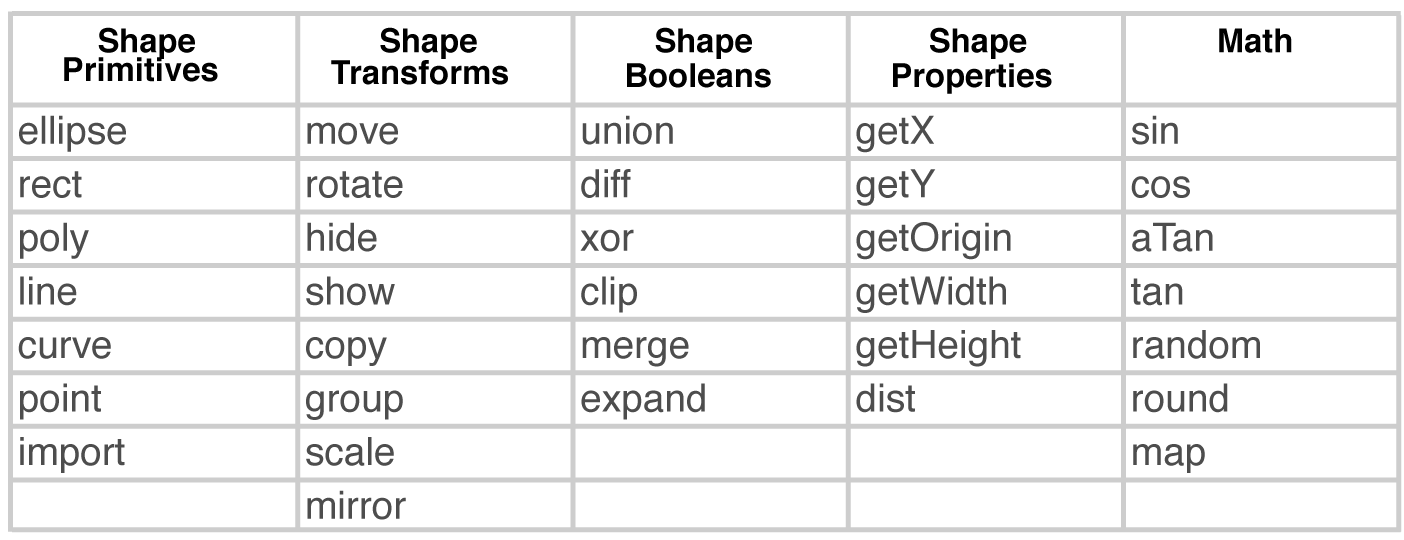
\includegraphics[width=6.5in]{images/api_table.png}
\caption{A selection of methods from the DressCode API}
\label{fig:api_table}
\end{figure}
\end{center}
\paragraph{Shape Primitives:}
DressCode shape primitives currently serve as the primary means of drawing (figure: \ref{fig:shape_primitives}.) The simplest primitive is a point, initialized two numerical parameters that denote the x and y coordinates. All closed-shape primitive methods (ellipses, rectangles and polygons) require an argument of either two x,y coordinates, or a point. This coordinate defines the origin of the shape and determines where  the shape will be drawn on the canvas. Ellipses and rectangles have an additional two optional parameters which specify width and height. If only two arguments are provided, the ellipse or rectangle will be drawn with a default width and height; if three arguments are given, the width and height will be the same. Polygons also have two optional parameters following the x and y origin coordinates, however they specify number of sides and length of each side, rather than width and height. Lines can be initialized either as four numerical values, specifying start and end x and y coordinates, two points, or as a vector, with a origin point,  a magnitude, and a heading in degrees. Curves are defined by a set of four points or eight coordinates, which determine the start, first control point, second control point and end point of a 4-point bezier curve. One other method of primitive generation was added in at the request of some of our early users: vector paths stored in Scalable Vector Graphics (SVG) format can be imported and drawn in the DressCode environment, and used in conjunction with primitive transformation and boolean methods.  

 \begin{center}
\begin{figure}[h!]
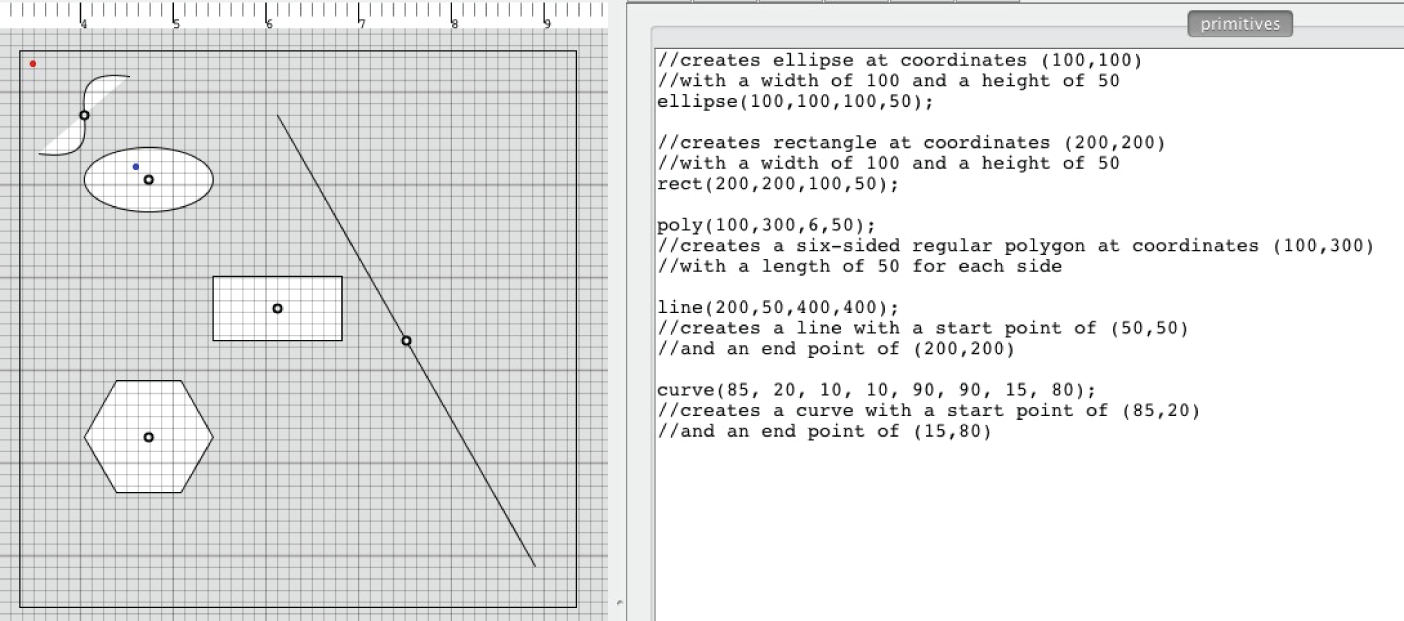
\includegraphics[width=6.5in]{images/primitives.png}
\caption{DressCode shape primitives with visible origins}
\label{fig:shape_primitives}
\end{figure}
\end{center} 

\paragraph{Shape Transformations:} \label{par:shape_transformation}
There is no required "draw" method for DressCode, as there are in many other graphics APIs, Instead all primitives are automatically drawn in the display panel in the order of their initialization, once the program has been run. In Soft Objects and Codeable Objects, when we required users to manually call draw method for any and all shapes in their program, they often forgot, and then had difficulty determining the reason why parts of their designs were not visible. 

Each shape primitive method returns an instance of the primitive it creates. A programmer can either create shapes with no reference as in figure \ref{fig:shape_primitives}, or they can assign them to an identifier at initialization, allowing them to reference and modify the shape later in the program. The shape transformation methods allow for a range of modifications to a shape, by passing a reference to the primitive the first argument, followed by different parameters for the modification, depending on the method (figure: \ref{fig:transformation}.) We began with a basic set of transformations, including move, rotate, methods that allowed for the modification of the stroke weight and color of the shape, and a hide method that prevented a primitive from being drawn. Based on our early user testing however, we gradually added in additional methods, based on what people wanted to do with their designs. This included a moveBy method, scale and mirroring functionality, a copy method, and an addition to the rotate method which allowed a shape to be rotated around a point other than its origin. 

 \begin{center}
\begin{figure}[h!]
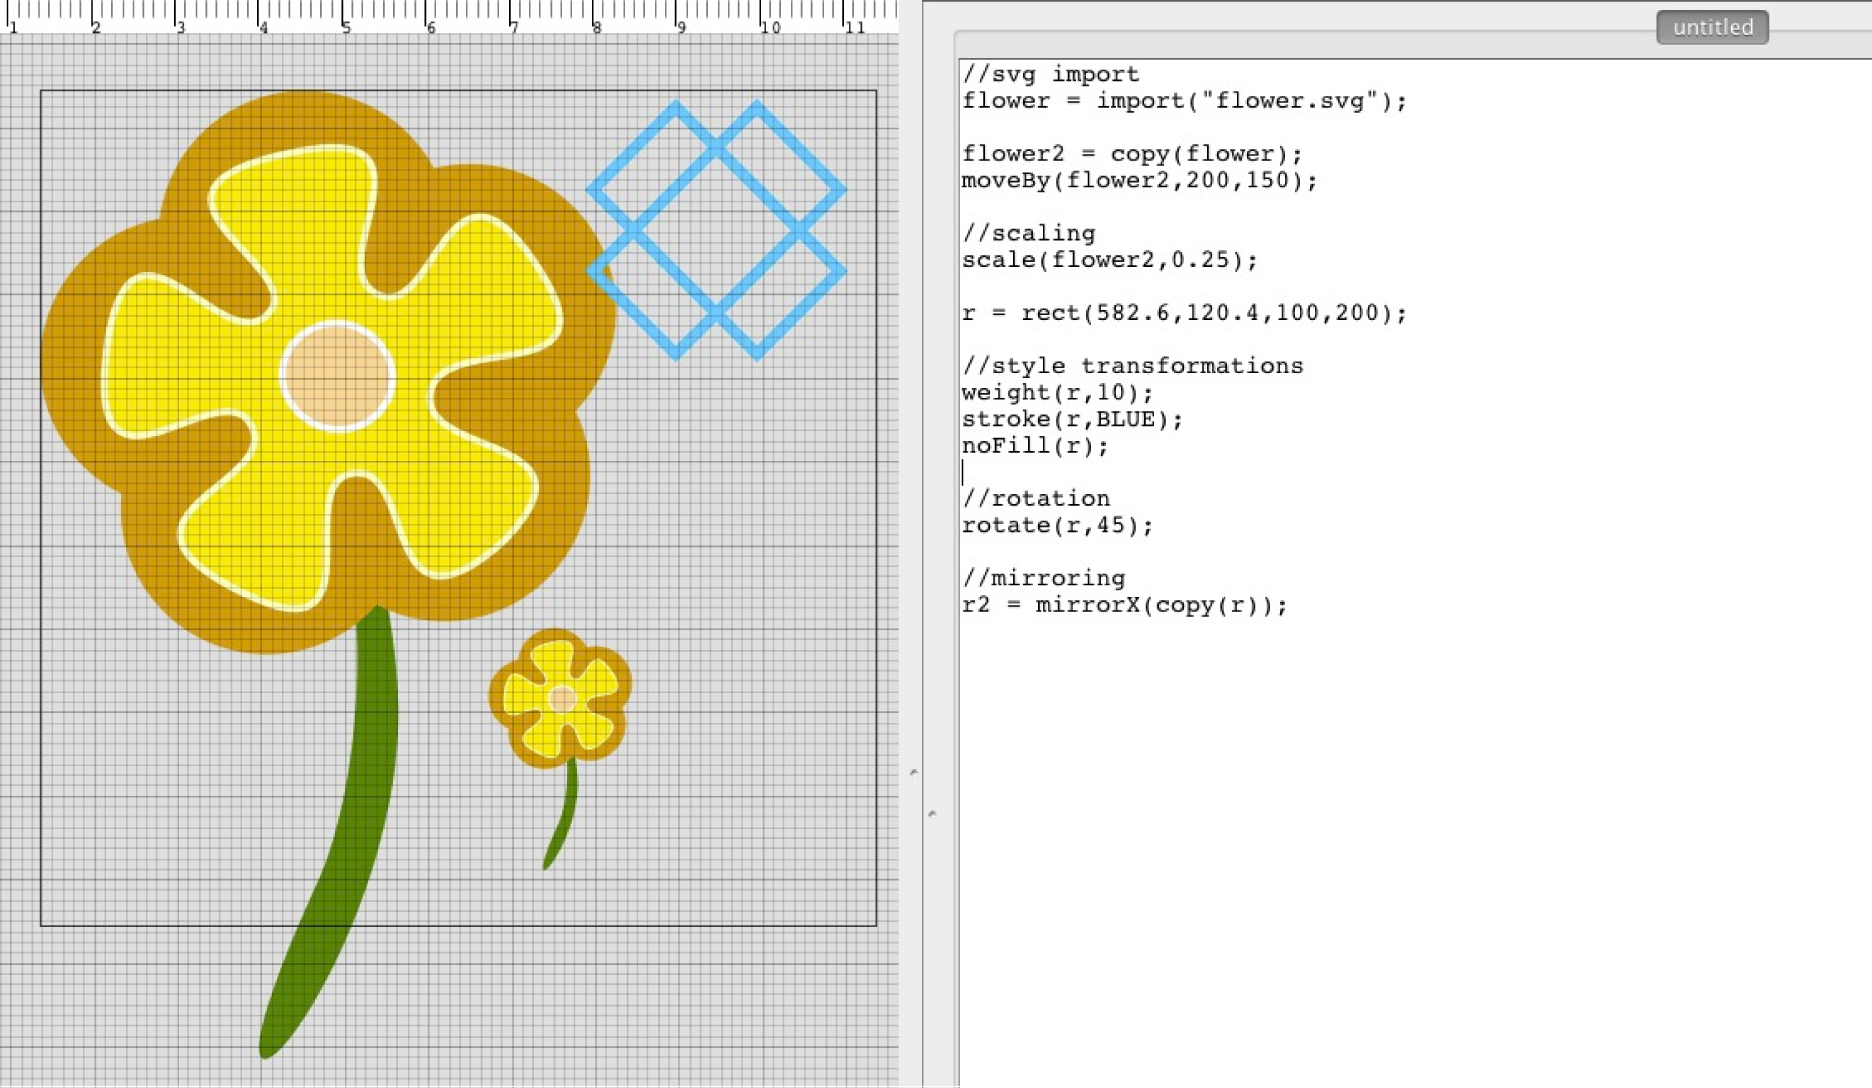
\includegraphics[width=6.5in]{images/transformation.png}
\caption{SVG import and sample of transformation methods}
\label{fig:transformation}
\end{figure}
\end{center} 

DressCode primitives can also be programmatically "grouped". Grouping provides an organizational structure for more complex configurations of primitives allows for the automatic transformations to multiple shapes. Groups have their own origin, which is used as the reference point for all move, rotation and scale methods applied to the group (figure: \ref{fig:grouping}.) For example, a collection of ellipses that is grouped and then moved to the center of the canvas would move the origin of the group to the center, and all the ellipses relative to the new origin. The origin of a group is automatically calculated as the centroid of all of the objects in the group and updated each time a primitive is added or removed. Groups are treated similarly to lists in that individual objects can be accessed and manipulated by via their index. Originally, primitives within a group were transformed relative to the origin of the group, however this caused confusion among many of our initial users. Each individual primitive is now translated according to the coordinate system of the canvas, regardless of whether it is in a group. 

 \begin{center}
\begin{figure}[h!]
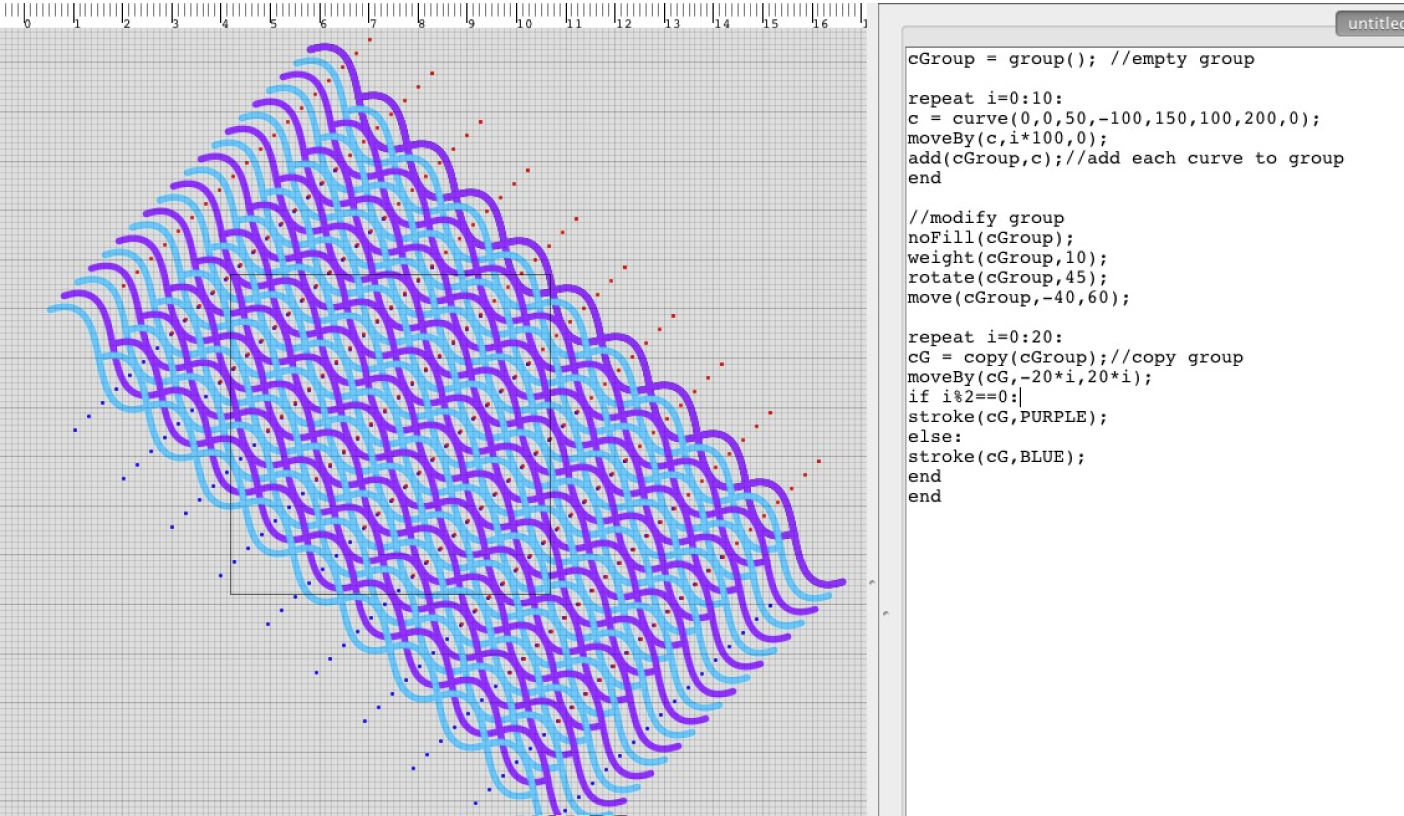
\includegraphics[width=6.5in]{images/grouping.png}
\caption{Grouping with transformation and repeat statements}
\label{fig:grouping}
\end{figure}
\end{center} 

\paragraph{Polygon Booleans:}
DressCode also features a subset of transformation methods for polygon boolean operations (figure: \ref{fig:boolean}.) The union, difference, exclusive or and intersection methods accept two primitives as arguments and return the corresponding shape, or group of shapes, depending on the operation. In addition, the merge method performs a union on all objects within a group and returns a single primitive. The expand method converts an object's stroke to a filled polygon with dimensions that match the weight of the stroke. The boolean methods were added for multiple reasons. Polygon boolean operations play an important role in CAD design for fabrication, because they allow for the creation of vector paths that appropriate for subtractive manufacturing processes. In particular, the merge method can function as a catch-all method for preparing designs for fabrication, and the expand method is useful for converting line drawings to paths that will retain their appearance when cut. In prior workshops, we relied on illustrator to prepare file paths for manufacturing, which was difficult, time-consuming and a hindrance to the computational design process. By integrating boolean operations as a part of the programming language in DressCode, it not only prevents users from having to rely on multiple software tools to design, but allows booleans to be used in a computational context, facilitating the creation of a whole new range of forms with simple primitives. 

Both the syntax and functionality of the boolean operations have been modified significantly since the first version of DressCode. In early versions, the majority of the booleans were expressed through mathematical notation, rather than with built in functions (e.g. ellipse1 + ellipse2 would perform a union). After some of our early user testing however, we depreciated this syntax, because many testers felt that mathematical notation was not intuitive beyond the union and difference operations. In addition, the mathematical notation required that all booleans be set equal to an identifier  (e.g. ellipse1 + ellipse2 = e3), in order to evaluate as a valid statement. The new method syntax still returns a resulting boolean, but can also be called without a corresponding assignment statement. Semantically, we originally had the boolean statements operate in a destructive manner as is the case in many graphic drawing programs; union(ellipse1, ellipse2) would destroy the original two ellipses and set the identifier ellipse1 equal to the resulting boolean. This was confusing however, because in a imperative program, the programmer could still reference the destroyed ellipse2. What we opted for instead, was a non-destructive boolean method wherein union(ellipse1,ellipse2) would return a third shape, which would automatically be drawn on the screen, and could be assigned to an identifier as needed. The original ellipse1 and ellipse2 would be hidden, but could both still be referenced without conflict, and could be revealed again on the canvas with the show() method. 

 \begin{center}
\begin{figure}[h!]
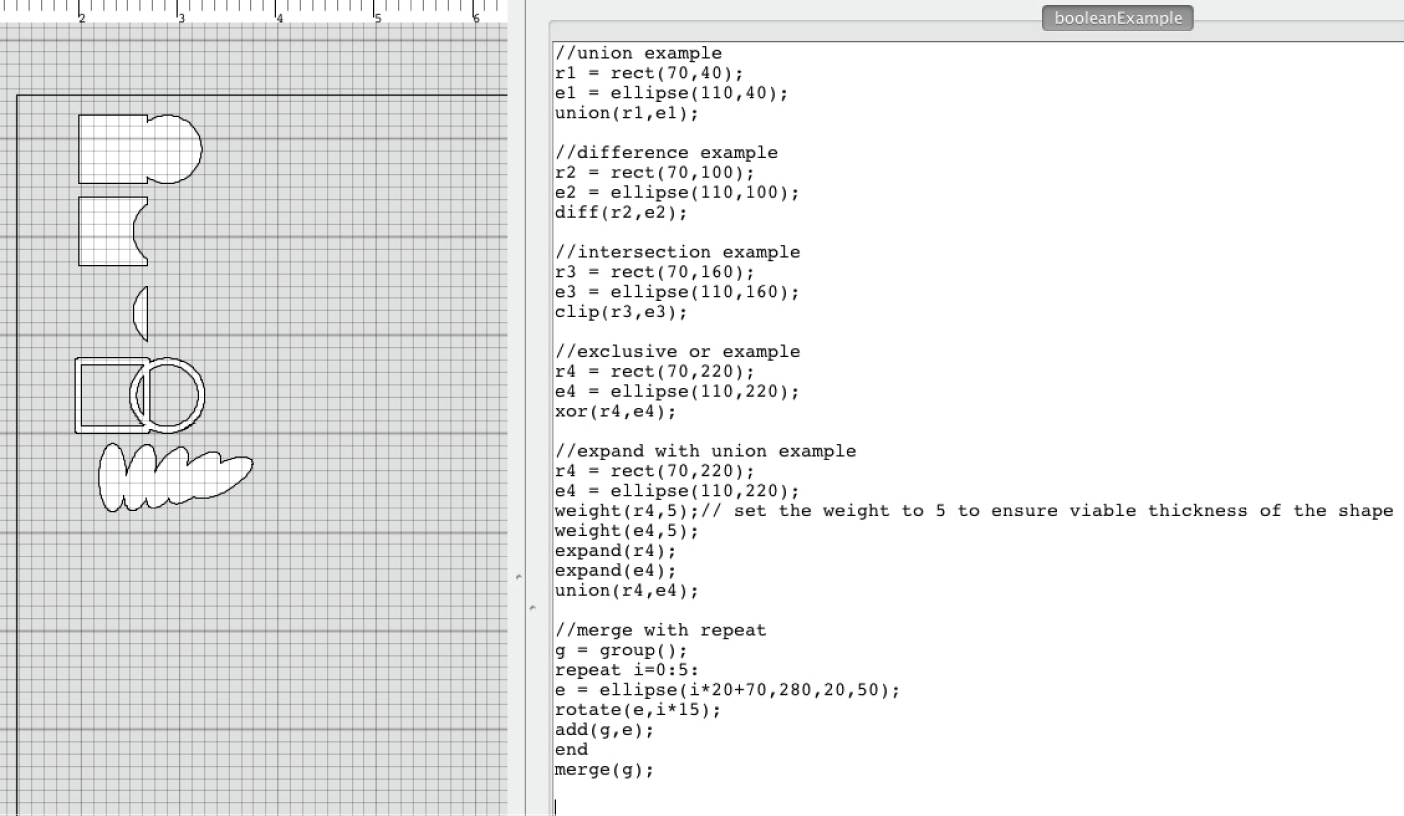
\includegraphics[width=6.5in]{images/boolean.png}
\caption{Polygon boolean operations}
\label{fig:boolean}
\end{figure}
\end{center} 
\paragraph{Additional Methods:}
Aside from methods for shape generation and transformation, DressCode features a set of getter methods that return information about a shape primitive, including its location, origin point, width and height, as well as a method to determine the Euclidean distance between two objects. There are also a set of methods that enable more advanced mathematical operations, including trigonometric functions, mapping, rounding and random number generation. The random method posses an interesting questions for implantation, as it generates different numbers each time a a program is run. This can be a useful design feature, allowing for the generation of numerous patterns with random variations. Figure \ref{fig:random_symmetry} demonstrates variations of an algorithm that produces randomly symmetrical stripe patterns.  It can also become problematic however, when the user wishes to keep the same randomly generated number for each interpretation of their program.  Finally, we recently added a set of methods that allow the specification of numerical values in inches, centimeters and millimeters, or in the current units of the drawing board. These methods are helpful when sizing and transforming primitives to real world measurements rather than pixel values.  

\paragraph{Constants:}
DressCode has a small set of constants to assist with design. WIDTH and HEIGHT correspond to the width and height of the current drawing board. PI corresponds to the numerical Pi value. Lastly, there are a set of color constants; RED, GREEN, BLUE, PURPLE, PINK, etc., that can be used to define the color of objects with fill and stroke methods. Custom colors can also be specified with 0-255 RGB values. 

 \begin{center}
\begin{figure}[h!]
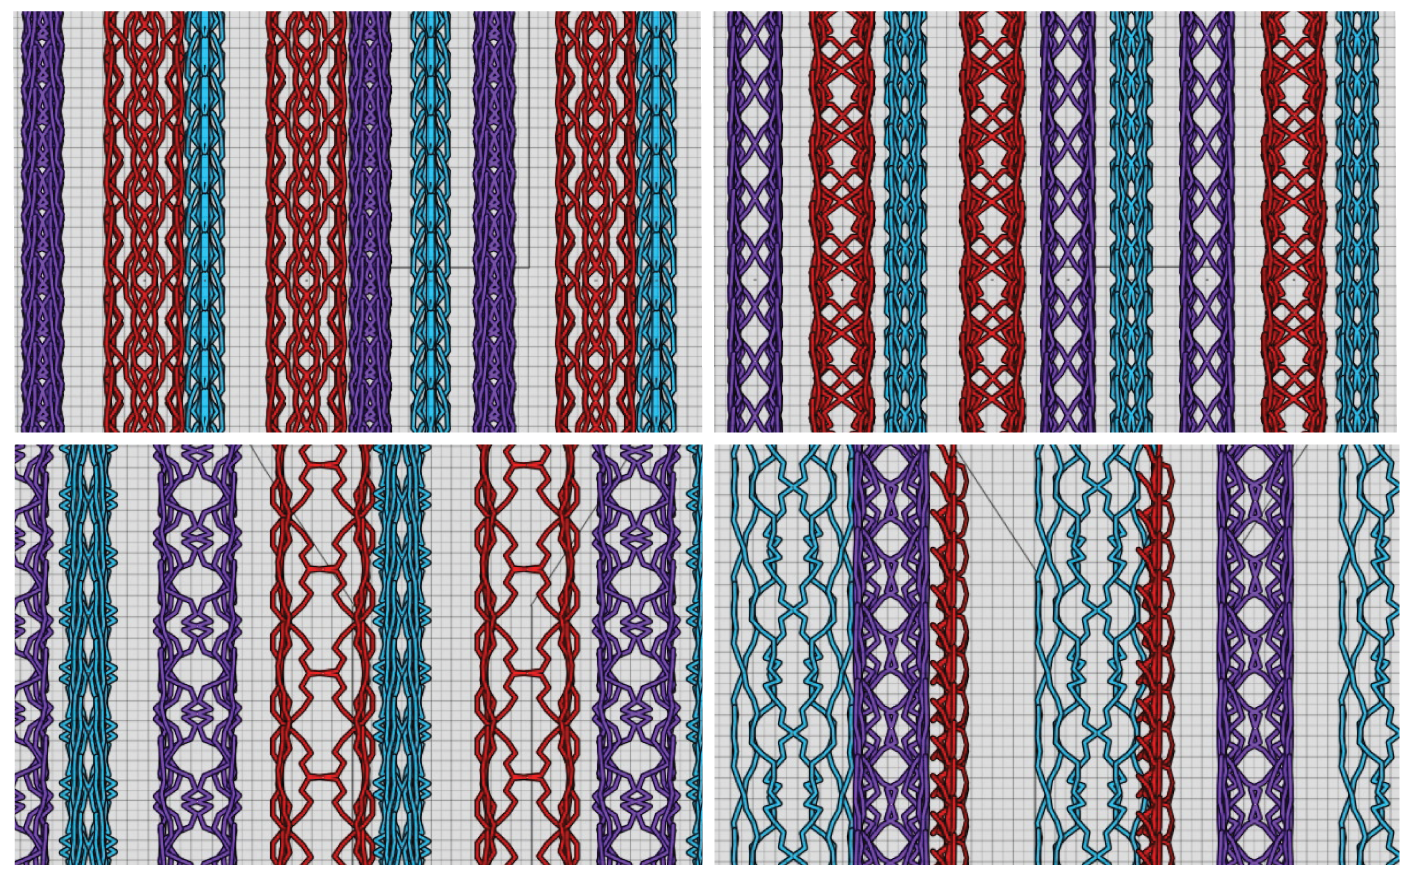
\includegraphics[width=6.5in]{images/random_symmetry.png}
\caption{Stripe pattern variations using the DressCode random method }
\label{fig:random_symmetry}
\end{figure}
\end{center}

\section{Fabrication and Crafting Process}
Similar to the prior tools described in this thesis  once a design is exported from DressCode, it can be imported to the control software of any 2-axis fabrication machine and fabricated into a set of parts.Depending on the material and fabrication process, a variety of end products are possible. In the process of protopying DressCode, I experimented several different fabrication machines, crafting techniques and artifacts. I tested DressCode primarily with the laser-cutter, however I also used it with more accessible machines including low-cost craft vinyl cutters and inkjet printers. I also examined sending DressCode files to online fabrication services such as Shapeways and SpoonFlower, to produce 3D-printed jewelry and larger inkjet printed garments.  I tested the resultant pieces from these fabrication processes with different crafting techniques that ranged in difficulty. Highly accessible techniques included making artifacts that required basic paper-folding or iron on appliqu�s for clothing. More difficult techniques included sewing garments, screen printing onto fabric, and jewelry making. There was frequently correlation between how easy a craft was to create, and how well it corresponded with the DressCode design process, indicating that for more sophisticated crafting processes like sewing, more advanced organizational functionality might be required for the DressCode software. 

To provide some support in the crafting process for independent users, my undergraduate research assistants and I created a set of example templates in DressCode that are directed towards specific end projects and fabrication machines (figure: \ref{fig:dresscode_examples}). We also began documenting some of the crafting techniques required to complete these projects online \cite{thesis_website}. Mainly though, I relied on in-workshop instruction or curriculum development to assist people in using DressCode to complete finished artifacts.

 \begin{center}
\begin{figure}[h!]
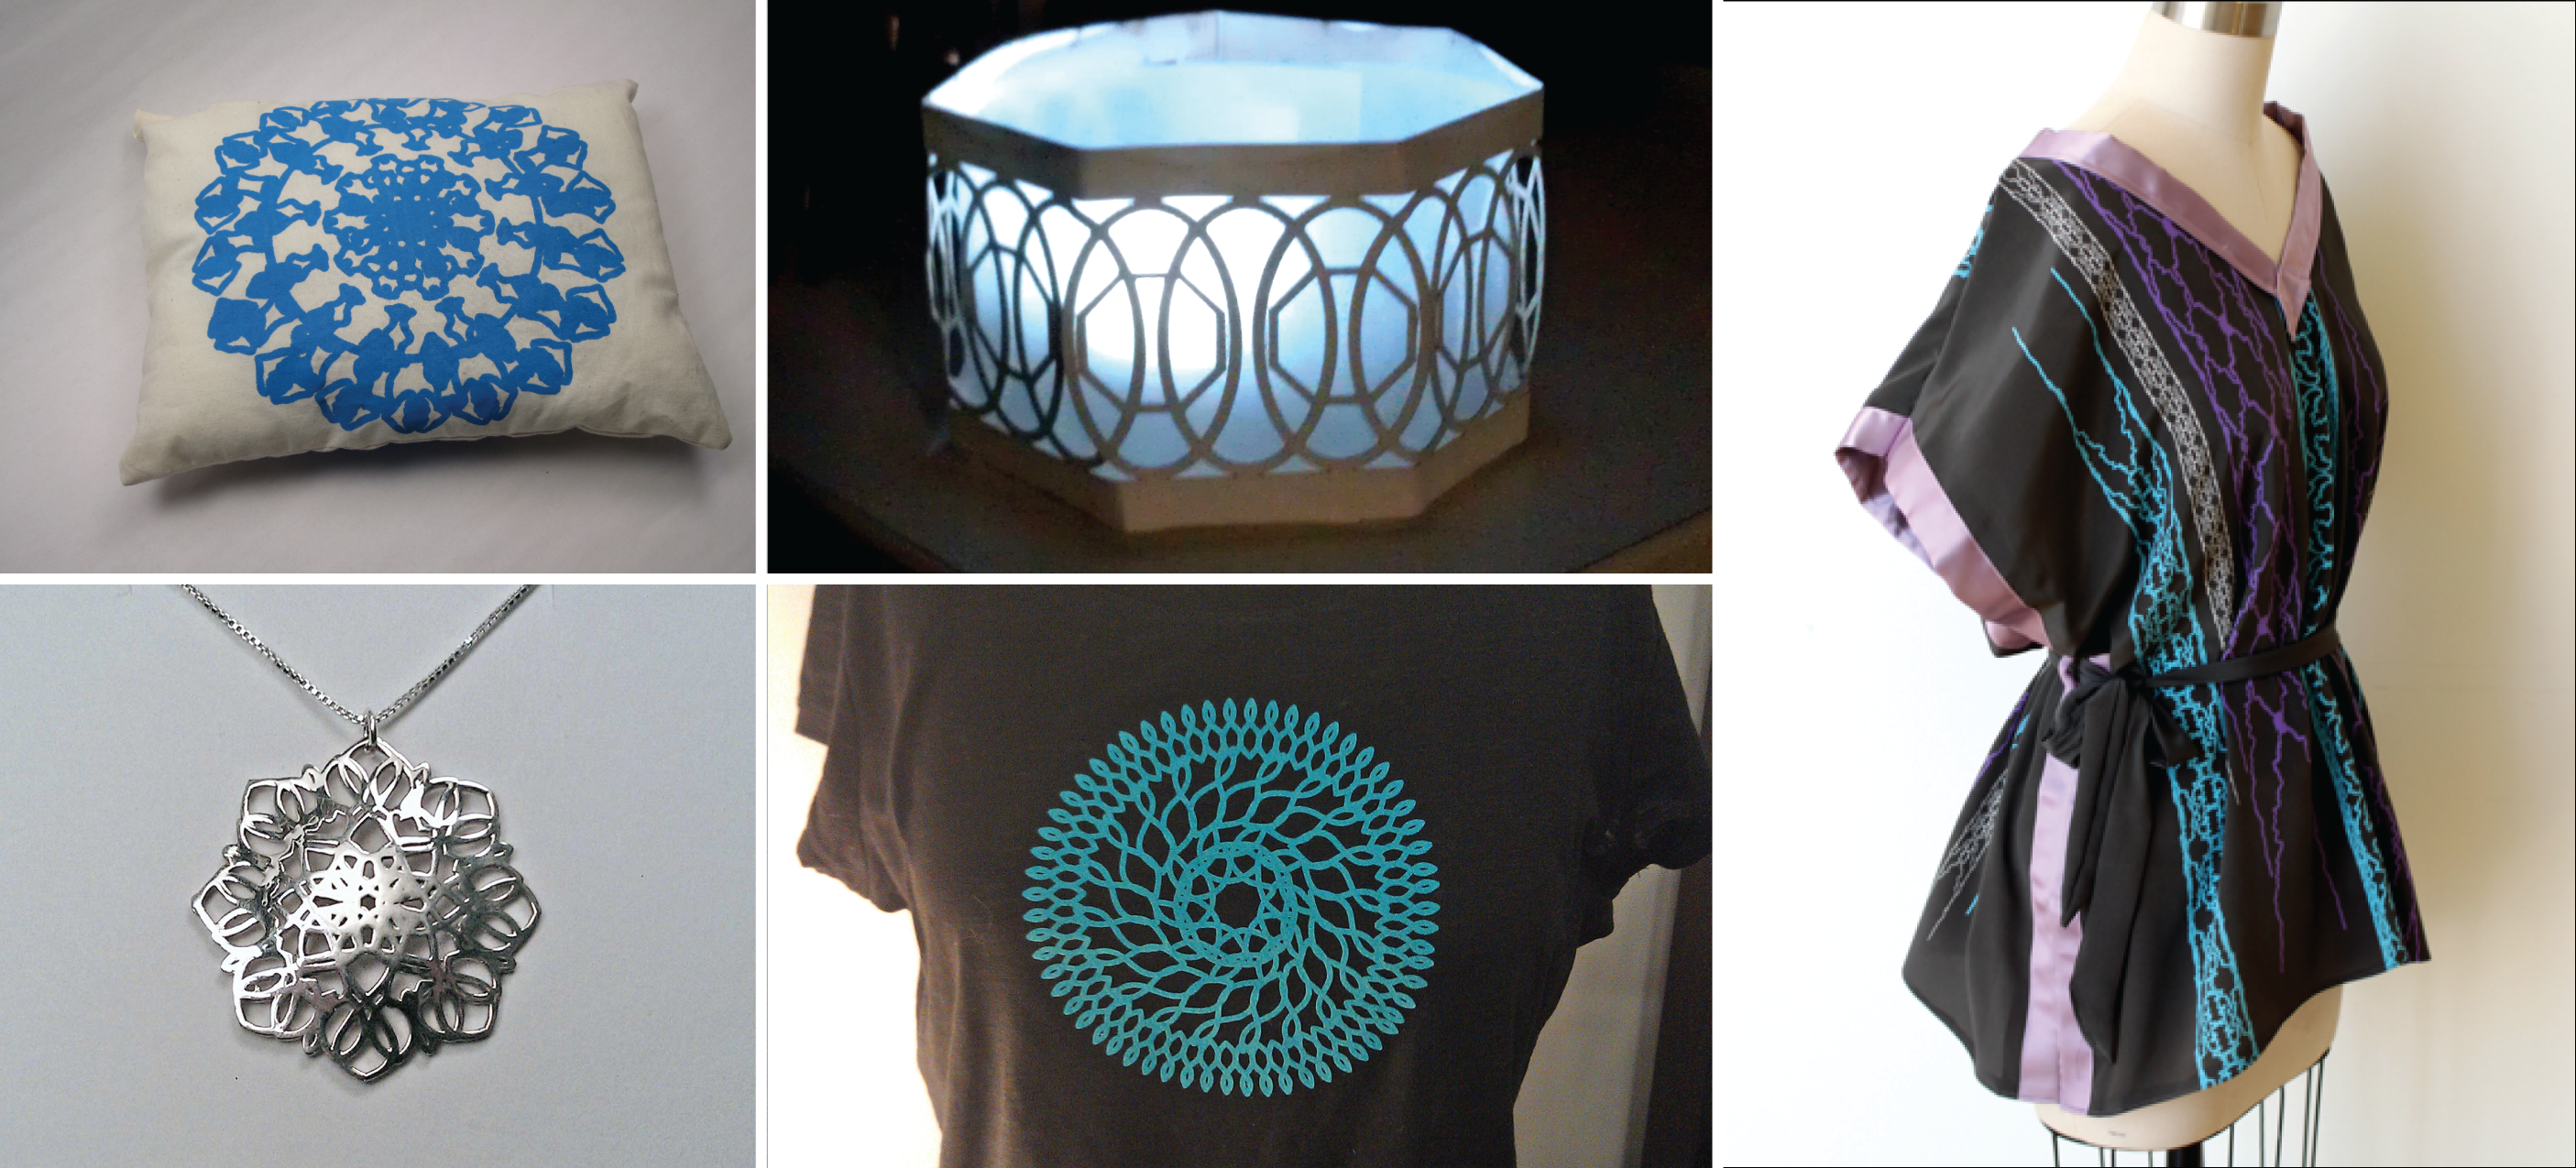
\includegraphics[width=\columnwidth]{images/dresscode_examples.png}
\caption{Several example artifacts created with DressCode Designs (clockwise from top left: vinyl-cut screen printed pillow, vinyl-cut tea light, ink-jet printed silk caftan, laser-cut iron-on tshirt, 3d printed silver pendant) }
\label{fig:dresscode_examples}
\end{figure}
\end{center}


\section{Workshops}
We informally tested DressCode with members of the FUSE development team, and by the staff at Dream Yard, an after school STEM education space in the Bronx. Following these tests, and a period of additional development, DressCode was evaluated during two separate day long workshops at the MIT Media lab. The first workshop was conducted among experienced designers, artists and programmers, who were selected individually from MIT, Harvard and the Cambridge community. The second workshop was conducted among ten young adults selected from youth organizations in Cambridge and art and craft workshop mailing-lists at MIT.Both workshops used DressCode to create laser-cut leather crafts.

\subsection{Expert Workshop}
The expert workshop was comprised of eight participants between the ages of  19 to 33. Five of the eight participants were female and three were male, and all had prior experience in programming. 75\% of the participants indicated a strong prior interest in design, and 50\% enjoyed crafting. All participants had formal training at a college level in either art, design or computer science 

The expert workshop was deliberately open and informal. We began the workshop with an open 30 minute discussion on the connections and intersections between design, arts and crafts and programming. Following this discussion the, participants were given a 45 minute general tutorial on the basics of the DressCode environment and programming language, after which participants were given access to the DressCode online code reference and a physical handout with quick references for some of the key methods. We also provided with a leather bracelet template and several example programs that generated different patterns for the template as  examples. Participants were given the option to design within the template or rely on modifying these examples, but were also free to create whatever they wanted.  Following the programing tutorial, participants were shown the basic fabrication process, and introduced to the materials, consisting of several varieties and colors of leather. Participants then had 3-4 hours to design their piece. As they completed their designs, they were taken in groups to the shop to fabricate their parts and then given access to craft tools and a variety of fasteners (snaps, rivets and jewelry connectors) to convert them into finished artifacts.

\begin{center}
\begin{figure}[h!]
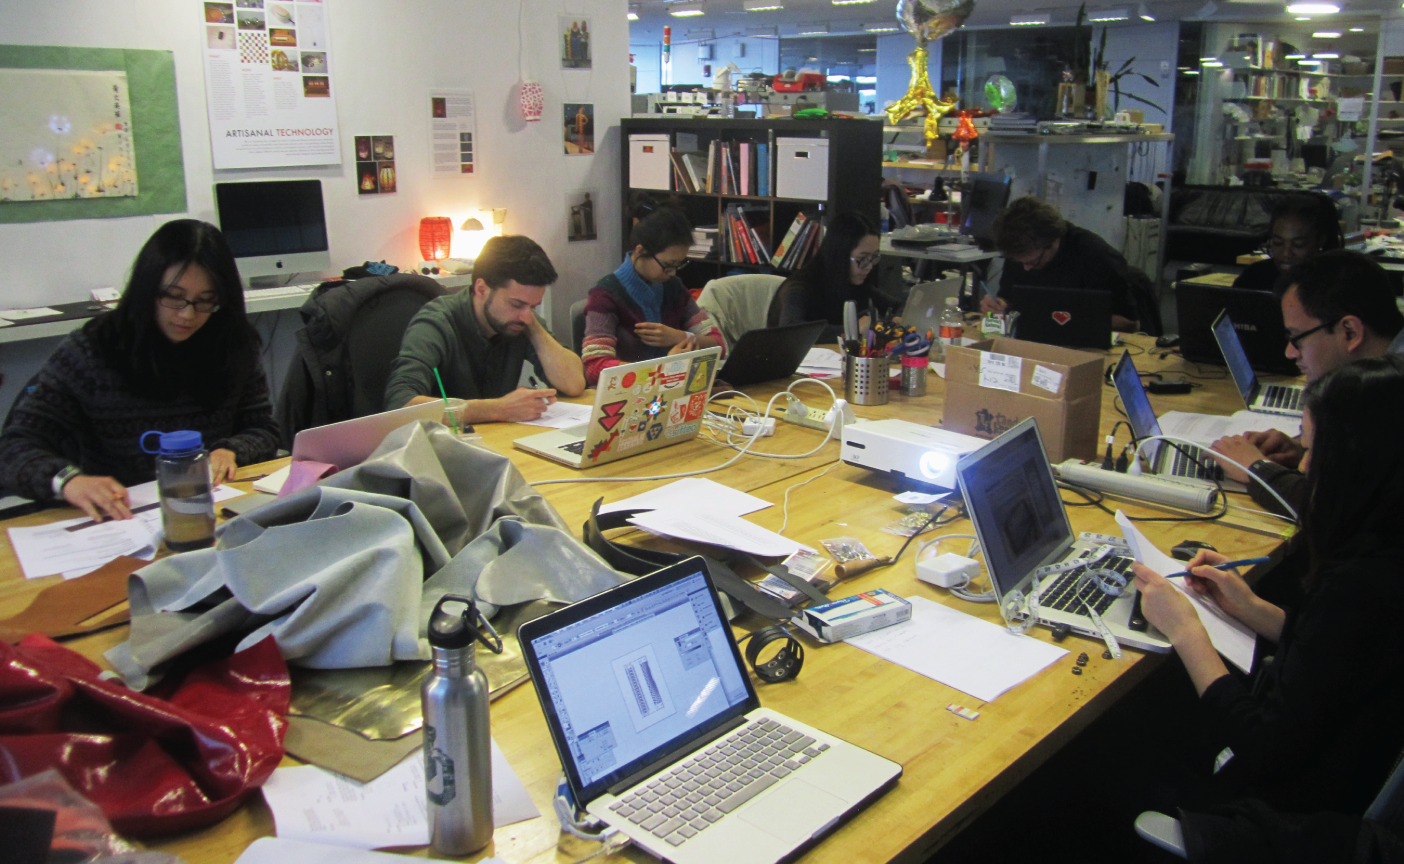
\includegraphics[width=\columnwidth]{images/adult_design_time.png}
\caption{The expert workshop}
\label{fig:adult_design_time}
\end{figure}
\end{center}

\subsection{Youth Workshop}
The youth workshop was conducted among ten young adults, aged 15-17, 20\% male and 80\% female. Five of the youth participants were participants in the Teach to Learn, Learn to Teach program in Boston \todo{cite program and find a description}. Of those surveyed three participants had prior experience with Scratch, and two had worked with the Arduino programing environment in a prior Media Lab workshop.  All of the participants said they had some prior experience in art, design, or craft.  Prior to the workshop, 60\% of the participants indicated that they did not feel comfortable programing on their own, however the majority indicated that they were interested in learning more about the process. 

The youth workshop was more structured than the expert workshop with the goal of helping to familiarize participants with the possibilities and affordances of computational design and fabrication. We began by passing out three colors of post-its for the categories of of art and craft, design and programming. We then held a 5 minute brainstorm where we asked each participant to write down people, tools, ideas and projects the associated each category on the respective colored post-it. After, we collected the post its, and put them up on a board in related clusters, and used the resulting associations to instigate 30 minute discussion on the participants ideas about the connections between the three domains.  We ended the discussion by talking about some of the possible craft applications of computational design, and began the introduction to DressCode.

\begin{center}
\begin{figure}[h!]
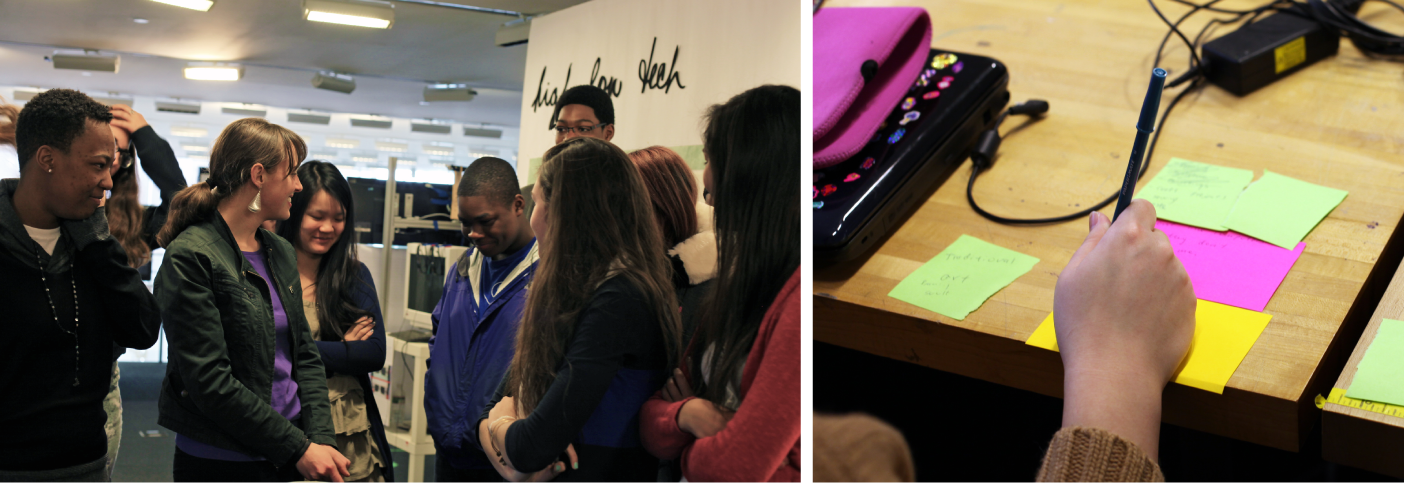
\includegraphics[width=\columnwidth]{images/youth_brainstorm.png}
\caption{The youth brainstorm and discussion}
\label{fig:youth_brainstorm}
\end{figure}
\end{center}

All of the design work in the youth workshop was structured around the concept of radial symmetry. I chose radial symmetry because it is a relatively easy pattern express mathematically, it serves as an excellent motivation for using a loop, and it is a pattern that is commonly found in nature, making it possible to generate designs that are floral,biological or organic in appearance. In addition, radially symmetric forms are often aesthetically appealing to people.  To begin, I explained the concept of DressCode and then spent 20 minutes leading the group, step by step through the process of creating a basic algorithm that used a repeat loop to create and rotate a number of ellipses around a central point (figure: \ref{fig:starting_algorithm}.) After every participant had successfully created their version of the algorithm, I showed them how they could use the same algorithm to create different designs by changing the number of iterations of the loop, the type of shape that was drawn, and the width and height of the shape. Participants then had 15 minutes to experiment with different parameters, and produce different designs, followed by a group show and tell session (figure: \ref{fig:show_and_tell}.) 

\begin{center}
\begin{figure}[h!]
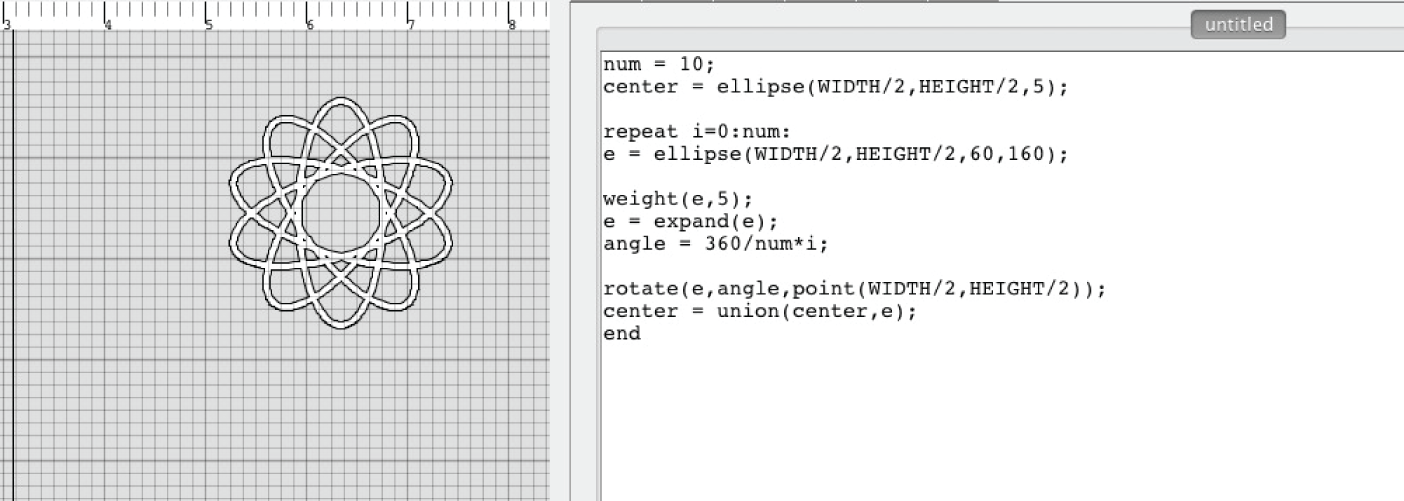
\includegraphics[width=\columnwidth]{images/first_algorithm.png}
\caption{The first algorithm learned by the youth participants}
\label{fig:starting_algorithm}
\end{figure}
\end{center}

\begin{center}
\begin{figure}[h!]
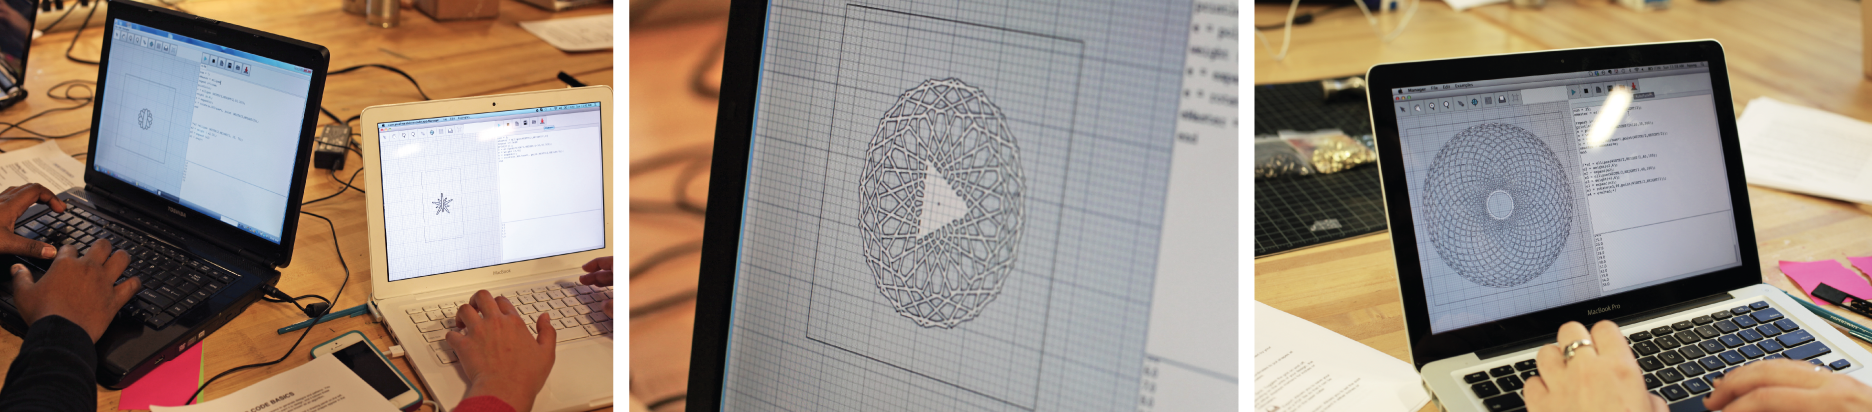
\includegraphics[width=\columnwidth]{images/show_and_tell.png}
\caption{Some example variations on the first activity}
\label{fig:show_and_tell}
\end{figure}
\end{center}

Next, the participants were provided with example programs that contained a bracelet template. The example programs featured a pre-written function that duplicated the algorithm they had written in the previous activity, with arguments corresponding to same values they were manipulating before. Participants were then given time to use the function to make multiple elements of the original radial pattern with different parameters. A second tab in the example program revealed the code for the radial function, which they could modify if they desired. The example template was constrained so that the dimensions of the bracelet would automatically correspond to the size of the drawing board. By measuring their wrist and resizing the drawing board, they could generate a bracelet of the correct size, and maintain their original design (figure: \ref{fig:bracelet_template}.)

\begin{center}
\begin{figure}[h!]
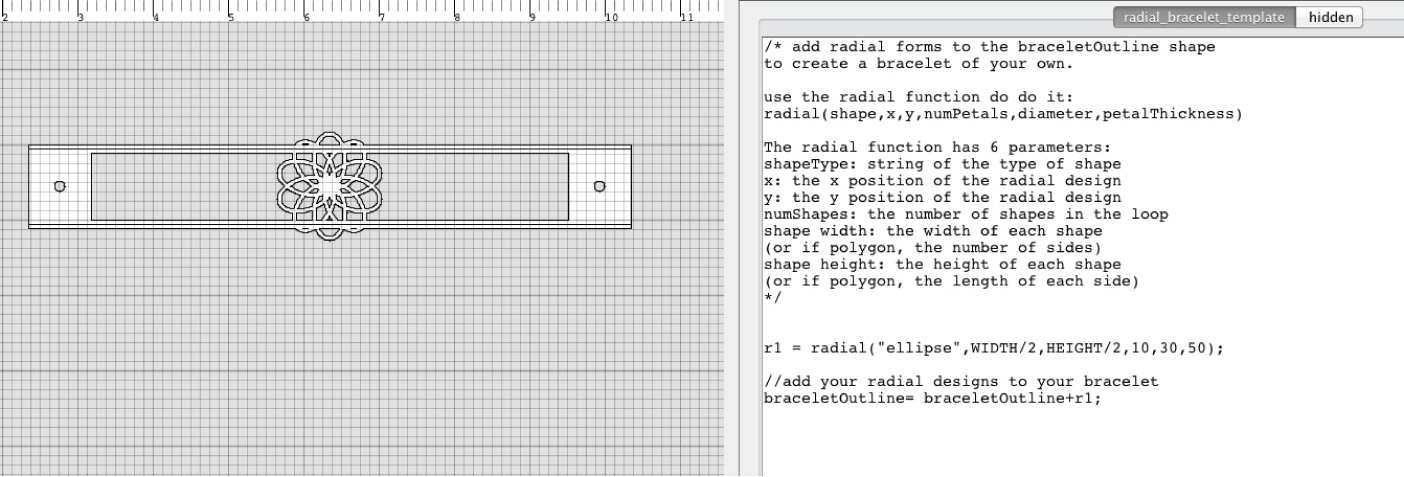
\includegraphics[width=\columnwidth]{images/bracelet_template.png}
\caption{The bracelet template with one instance of the radial function being called}
\label{fig:bracelet_template}
\end{figure}
\end{center}

Participants were given approximately two hours of free design time. When they had settled on a final design, they first printed out a paper copy and ensured that it fit their wrist. Following that, they selected their material and were taken in groups to the laser cutter where they cut their piece. Afterwards, they were shown how to attach the fasteners to the bracelet, and provided with additional handcrafting tools that allowed them to further alter the piece by hand. 

\section{Results}
\subsection{Expert Results}
All but one participant in the expert workshop indicated that they were able to successfully able to complete a finished product. The types of end products varied.  While most participants produced leather cuffs, people also created finger puppets, earrings and a belt using the software. Many participants also mixed materials and techniques and created There was a high degree of variation in the algorithms used to create the finished products. Several participants relied exclusively on the radial symmetry algorithm, but others created patterns with computationally ordered curves, rectangles and lines in different arrangements.  The participant who created the leather belt designed the pattern so that it demonstrated the evolution of the algorithm that comprised it; as the individual patterns progress across the length of the belt, they grow in complexity. Because of the high degree in variation among approaches and end products, conducting the expert workshop was difficult. Many of the participants began with design goals that were at odds with the affordances of DressCode, such as creating representational characters in the case of the finger puppet example, or creating organic, irregular forms.  In addition, several of the end projects required instructor intervention to ensure they were suitable for fabrication. Overall, the expert workshop produced a promising set of results and demonstrated the limitations and benefits of using DressCode across a broad range of design approaches. The expert participants also provided feedback on specific features to incorporate into future versions of the DressCode software. The random method and unit conversion methods were added directly following the workshop based on participant suggestion.

\begin{center}
\begin{figure}[h!]
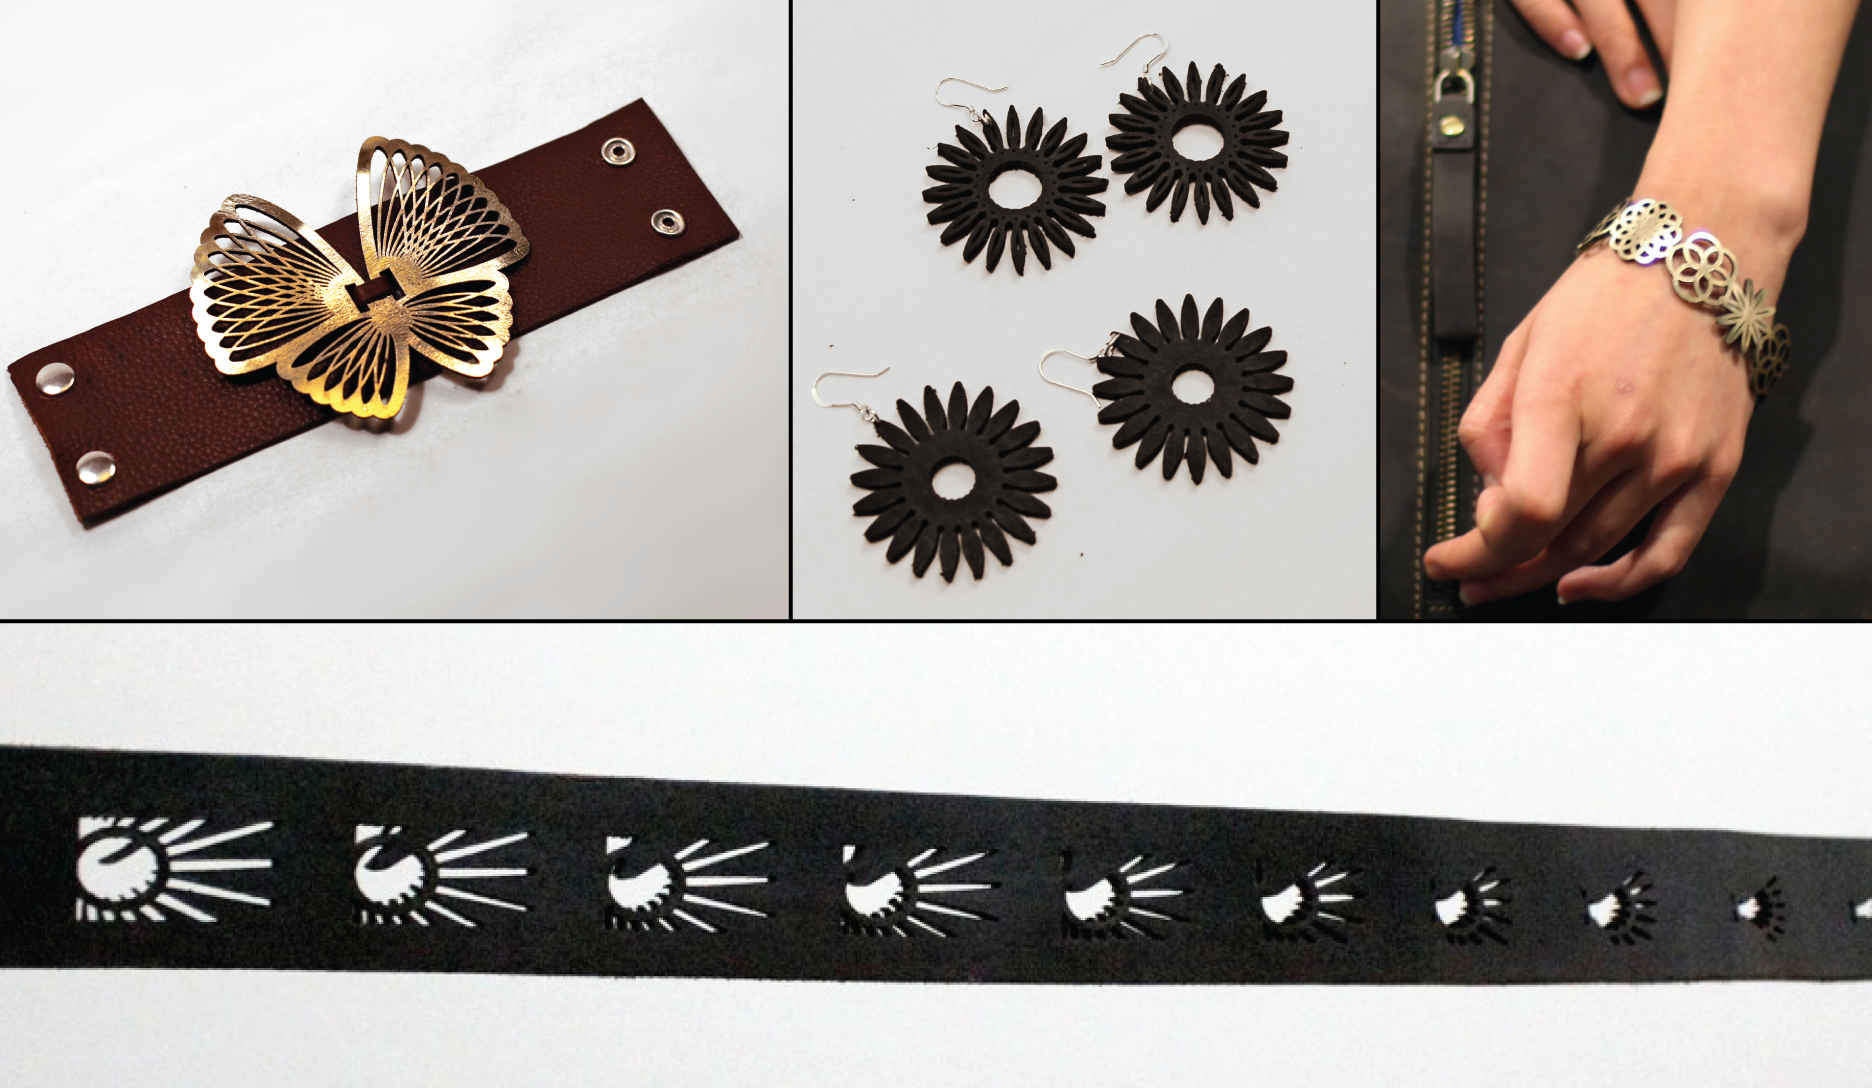
\includegraphics[width=\columnwidth]{images/expert_results.png}
\caption{a sample of the completed projects from the expert workshop (clockwise from top left: butterfly cuff, leather earrings, patent leather bracelet, algorithmic progression belt)}
\label{fig:expert_results}
\end{figure}
\end{center}

\subsection{Youth Results}
The youth workshop was more structured than the expert workshop, and produced a more consistent set of physical products as a result. All participants in the youth workshop were successfully able to use DressCode to produce a unique leather cuff (figure: \ref{fig:youth_results}.) Despite the consistency in form, the patterns and approaches among the resulting bracelets were highly varied. Each participant was also able to successfully write their own radial symmetry algorithm in the initial lesson and produce a variety of patterns with it. During the bracelet design portion, several participants directly modified the algorithm in the template to better fit their design goals, however all participants primarily relied on radial symmetry in their bracelet design. Eight of the participants  said they planned to wear the bracelets they created during the workshop, however two indicated that they planned to give them as gifts, rather than keep them for themselves. A comparison of the pre-and post-workshop surveys showed that several of the participants' comfort in programing increased following the activity. In addition, more participants indicated that they thought programing was a good tool for personal expression, and design respectively and all participants stated that they believed they could use programing to make things that were beautiful, whereas several had disagreed with this statement before the workshop.

\begin{center}
\begin{figure}[h!]
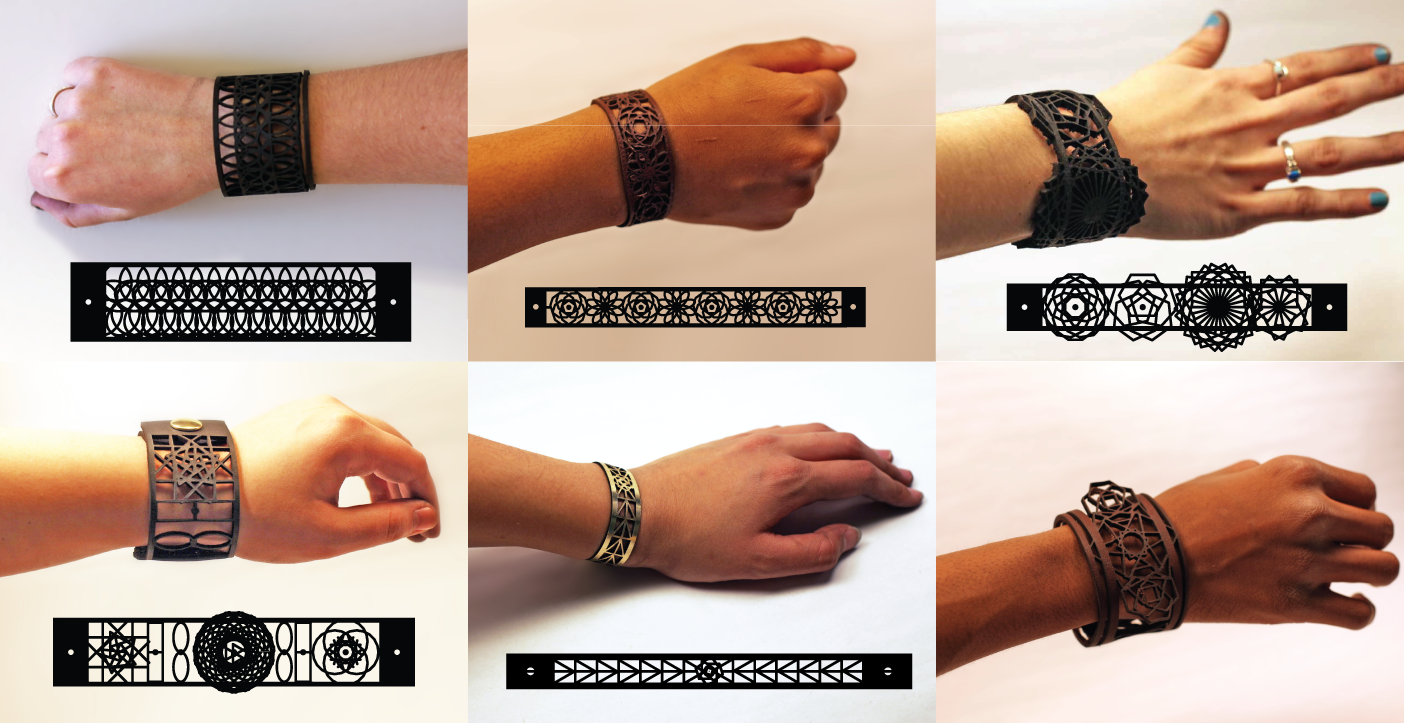
\includegraphics[width=\columnwidth]{images/youth_results.png}
\caption{a sample of the completed leather cuffs from the youth workshop}
\label{fig:youth_results}
\end{figure}
\end{center}
\section{Curriculum description}
\section{Preliminary curriculum results}
\section{Discussion}

\subsection{Starting notions of craft and computation}
When developing a tool for combining craft and computation, it is important to understand people's prior conceptions of these domains. In the case of the DressCode study, there was a strong distinction between the views of the two groups of participants on the respective roles of craft and computer science. During the expert discussion, two separate forms of craft were discussed. The first referred to craft as hobby and amateur practice. The experts also demonstrated an appreciation for craft as an artisinal practice, wherein handcrafted artifacts held higher value than mass produced ones because of the time and expertise required for their production. In the youth discussion of craft, the recognition of craft as artisanal practice was completely absent. Instead they referred to craft as an recreational activity, that anyone could do. The perception of craft as open and accessible by young people is encouraging, however many youth participants also dismissed the difficulty of craft in comparison to programing. One young woman articulated her view on the difference between writing a program and throwing pottery, stating that she knew she could throw a pot, but that she would be unable to write a program, despite having no prior experience in either medium.  The variation in expert and youth perspectives on the levels of expertise present in craft is understandable, given the educational differences between the two groups. 

There was also a difference between the amount of variation in the crafting processes between the two experts and young people. Several participants in the expert group experimented with layering different materials on top of one another for a different effect. One participant sewed a portion of her project rather than attach portions with snaps. Another used the snaps as an aesthetic component, by placing them across the length of the piece and then snapping on different colored pieces of leather in different patterns. There was limited variation in the approaches the youth practitioners took in the crafting portion. Furthermore, many of the youth participants remarked on the surprising difficulty of the handcrafting component.

\begin{quotation}
\textit{``Something that was difficult was hammering the snaps in straight enough for them to function well."}
\\Youth Participant F

\textit{``It was enjoyable being able to wear it and making sure that it would fit. It was a little stressful figuring out how to put the clasp on. "}
\\Youth Participant K

\textit{``I think the actual physical copy [of my bracelet] is slightly less attractive than the one I had on the computer."}
\\Youth Participant C

\textit{``I hate being anxious because I don't know if it's going to come out right. I like the designing on the computer, but once it comes out it looks like crap. So I'm really happy that I came to this (workshop), this is the first one that came out."}
\\Youth Participant ST

\end{quotation}
\begin{comment}
continued excitement w/ laser cutter
\begin{quotation}
\textit{``I was excited- I was really happy when it came out. Even though I've used laser cutters, the ones at our centers aren't powerful enough to do something like this.
This is probably the most complex thing that I've done with a laser cutter."}
\\Youth Participant ST
\end{quotation}
\end{comment}
It is likely that there is a connection between people's perception of craft, and their ability to engage in new crafting techniques, despite encountering difficulties along the way.
\todo{section currently not complete}
\begin{comment}
\begin{quotation}
\textit{``It's just a whole new program, it's not something that I already know how to do. Arts and crafts is like, anybody can do it, but here you need to follow what [the instructor] says, you need to know what you're doing ... I think you just need to have more fore-hand knowledge to know what to do."}
\\Youth Participant S.M.
\end{quotation}
\end{comment}

\subsection{Enjoyment in Programing}
One of the most important points of evaluation for DressCode was how successful novice programers felt in their attempts to use it. In the Soft Objects workshop, participants were excited about the potential of programing, but unanimous in their frustration in using traditional programing syntax with the Soft Objects library, and requiring instructor assistance to execute simple actions. It is difficult to evaluate the DressCode workshop parallel to Soft Objects because the DressCode workshop took place over a shorter time period in the context of a more constrained activity. When evaluated as an independent case of novice programing however, the response in the DressCode environment by novice programmers was promising. In general the youth participants expressed  a sense of enjoyment and low levels of frustration with the coding portion. When asked if they found the programing enjoyable, participants responded in the following ways: 

\begin{quotation}

\textit{``It wasn't as hard as i thought"}
\\Youth Participant 1271996 (survey)

\textit{``[It was enjoyable] because it was very straightforward to use and easy to understand."}
\\Youth Participant 091897x (survey)

\textit{``Yes, I didn't have much experience with programming before the workshop so it was fun to screw around and see if I could push the boundaries of what I could achieve by hand."}
\\Youth Participant 091897x (survey)

\textit{``[The] computer programing was enjoyable for me because i had wanted to do it before but never had the chance. so this workshop gave me exposure to something that i wanted to do for a while. and i totally loved it."}
\\Youth Participant 092297m (survey)

\textit{``I liked [the language], it wasn't tough, it was very simple. That barrier was removed for me so I could focus on the design."}
\\Youth Participant ST
\end{quotation}

It should be noted that the last quote was from a participant who had prior coding experience. All of the other quotes came from participants who were new to programing. Some of the participants did express difficulties, however they were often described in conjunction with enjoyment or with the the recognition that through some effort, they could be overcome:

\begin{quotation}

\textit{``The computer programming was enjoyable for me; however; it was a bit frustrating and confusing at times."}
\\Youth Participant 123097f (survey)

\textit{``It was fairly enjoyable, if arduous and frustrating. Once I figured out how to do it it wasn't too hard."}
\\Youth Participant 100397c (survey)

\textit{``It was alright except a bit hard to learn but once you know it its pretty much simple for the rest of the time."}
\\Youth Participant 05231997 (survey)
\end{quotation}

Other youth participants also elaborated on the ways in which they felt programing had been useful in the design process. Their responses  evoked some of the key affordances of computational design discussed in section \ref{sec:computational_design}. For example, one participant described the advantages of programing for creating precise design elements:
\begin{quotation}
 \textit{``Basically with programing, it like- say I wanted to draw it by hand with the mouse- it would be a lot harder to make the image um , perfect's not the word..everything was scaled perfectly. Say you wanted certain shapes to be certain angles or certain sizes, if you were to code it, you can get it at the right angle, where if you were to draw it by hand, you wouldn't know what angle it is."}
 Inteviewer:\textit{`` So the precision?"}
Youth Participant N: \textit{``Yes."}
\end{quotation}

The recognition of the ability to create complex designs through repeated simple actions was another common sentiment. Again from the interviews:
\begin{quotation}
\textit{``[My design] feels complicated and simple to me at the same time- it may seem simple to me because I know the rules behind it."}
\\Youth Participant R.
\end{quotation}

Participants also discussed the parametric qualities of designing with code:

\begin{quotation}
\textit{``[I liked] the programming part.. learning different strips of code and what they did, and just changing the basic codes they gave us so basically it looks more unique"}
\\Youth Participant N

\textit{`Something that was useful about using programming to design this bracelet was that it was easy to change the sizes of the shapes very quickly."}
\\Youth Participant 123097f(survey)
\end{quotation}

Responses like these suggest that DressCode was successful in introducing participants to some of the qualities of computational design, similar to the SoftObjects workshop. Perhaps the greater success was that participants were able to implement these qualities in a more independent manner than with Soft Objects, allowing for a greater sense of personal agency, and a broad appreciation of the power of computational design. This appreciation was indicated in part by the enthusiasm of the participants following the activity:

\begin{quotation}
\textit{``Now i know that you can use computers and programing and stuff to design pretty and physically appealing things, instead of just complex robots and stuff."}
\\Youth Participant 092297m (survey)
\end{quotation}

\begin{quotation}
\textit{``It was really fun and I gained a lot of knowledge from it- knowing how to program, knowing different types of ways to manipulate shapes and radials."}
\\Youth Participant S
\end{quotation}

\begin{quotation}
\textit{``[The bracelet]  is a physical manifestation of my success in coding, maths, and programatic design, and that's what I see when I look at it. It is a little coding confidence totem that can inspire me to continue developing my skills and passion in this area - wow, I didn't realise I felt that strongly about it!"}
\\Expert Participant 090585p (survey)
%(A participant speaking about making a design for  t-shirt with DressCode) \textit{``... it's not necessarily just making a shirt with the program, but when you combine this with the %program you get the shirt, so there's endless possibilities.''}
%\\Youth Participant R
\end{quotation}

These positive reflections on the potential of programing, combined with the appreciation of specific computational affordances in design, and feelings of accessibility and feasibility of the programming process, are encouraging for a day-long programing activity with first-time coders. An analysis of these successful results in the context of  the prior workshops with Soft Objects and Codeable Objects point to several distinguishing factors. The first is related to the feature-set of DressCode itself. Although the tool still shows significant room for improvement, it appears that the simplified programing syntax, improved drawing API, and more-immediate visual feedback accounted for some of the success of the activity. By providing the participants with a small set of useful programming methods that could be used to generate complex forms and patterns, textual-computational design became relatively feasible for novices. In addition, the features in DressCode that made the transition from design to fabrication less convoluted (by not requiring any post-processing), reduced the technical concerns of the participants and allowing them to focus on using programming to design, rather having to ensure their patterns would work in a practical sense.

Another key factor in the success of the activity was the structure of the workshop itself. By relying on radial symmetry as a design mechanism, participants were given a task that had a wide range of design possibilities, but only required them to understand a few key concepts. This differed significantly from using the Voronoi diagram in Codeable Objects- an algorithm that is easy to explain in concept, but extremely difficult to implement. It also differed from the approach of the SoftObjects workshop, where the wide variety of computational approaches made it difficult to simultaneously ensure that participants designs were successful and that people understood the algorithms behind them. When a longer-term workshop is conducted with DressCode, I will attempt to expand upon the constraints of the first workshop by selecting an additional set of algorithmic patterns similar to radial symmetry in simplicity and design feasibility. Patterns such as spirals, waves and basic fractals offer some possibilities, but there are many others.

One final element in the success of the DressCode activity was the presence of several well-prepared facilitators. For the workshop, I had four facilitators, including myself. The three additional facilitators had prior experience working with DressCode and were included in the development of the activity itself \footnote{It should be mentioned that I did have several wonderful facilitators for the Soft Objects workshop. Their presence was more sporadic however, and their involvement was not as deliberately planned as in the case of the DressCode activity.}. While a part of the facilitator assistance came in the form of addressing bugs and answering syntax questions, they were also invaluable in providing support in the design process. The other facilitators assisted participants by suggesting new design directions, helping them to evaluate their designs, and being supportive and encouraging throughout the day. Although it is desirable to strive for developing novice programing environments that allow for independent use, the benefit of well-structured in-person support should not be overlooked. Especially in the context engaging people first-time programing experiences with computational design, it is beneficial to have support staff who can simultaneously provide both technical and critical assistance. 

\subsection{Design Processes of Youth and Expert practitioners}
Because DressCode was developed to support personal visual expression through programing, a significant part of my evaluation focused on the design strategies that emerged through the use of the tool. The interviews and post surveys indicated that participants in both the expert and youth workshop engaged in a variety of design strategies in working with DressCode. When asked about her design, one young woman described a process of conscious planning. For example:

\begin{quotation}
\textit{``Well I wanted this one (pointing to an element of her bracelet) the first one made out of radial ellipses; I wanted it to look like a flower when they layer down, and the second one is kind of like the same thing, but I wanted to have the pentagon or hexagon, and the next one is the snowflake, and I wanted it to look like a snowflake because my favorite season is winter, the next one the center looks like a different sort of snowflake because all snow flakes are different, so I chose different shapes, and the last one is a rectangle-like a square in the middle and then it's like hexagons."}
\\Youth Participant S
\end{quotation}

She also described the activity as requiring ``creativity and thought and dedication", due to the high degree of complexity. When asked how she found programing useful in her design she said:

 \begin{quotation}
\textit{``You type it in and it brings it to life for you. You can do it on your own....you don't have to buy it. It's different than the casual way that somebody gets a bracelet."}
 \end{quotation}
 
Other participants also indicated that impromptu choices played a role in their final design, in combination with pre-mediated decisions:

\begin{quotation}
\textit{``A few days before the workshop, I was thinking about how I will not likely wear a leather bracelet, but a belt I would definitely wear. I didn't really have an idea for what kind of algorithmic design I wanted to make. During the discussion at the beginning of the workshop, somebody used the word "evolution," and I started thinking about making a design that repeats and gradually changes across the belt. I had a hard time coming up with an interesting shape with an interesting transformation. I started with a blossom of rectangles, and tried a bunch of variations. At some point somebody said it was like an animation, which gave me some positive energy in thinking about the design (and I thought I could be a human zoetrope, spinning in sync with a strobe). It started to get more interesting when I added the masking effect. I eventually made the individual pieces making up the ellipses instead of rectangles, which both made the thing softer, and emphasized the transition as they collide with the mask, forming sharp corners."}
\\Expert Participant 071279R (survey)
\end{quotation}

\begin{quotation}
\textit{``I saw that the duplication of a large shape was kind of happening with a lot of people's designs, so I decided to try and do something a little different. (Show's a first design (ellipses side by side on a line). That was the second phase of this, and then I just started screwing with numbers to see what I could get and I came up with this. I didn't know if I wanted the entire thing to be symmetrical or not, but then I thought that that was getting too boring (the symmetry), so then I changed the number of shapes in the loop to an odd number instead of an even one so that it would offset the design, and came up with this."}
\\Youth Participant R
\end{quotation}

\begin{quotation}
\textit{`I kind of like started off playing around with the main stuff and once I got that I narrowed it down and tried to switch around different parts to see which parts worked best."}
\\Youth Participant C
\end{quotation}

\begin{quotation}
\textit{`I used an example I liked and decided to spend time doing an earring or single pendant so I could focus on manipulating the example to see how the program worked. I also picked something that repeated the same unit for simplicity and the time limit."}
\\Expert Participant 081764
\end{quotation}

Youth and expert participants varied in the levels of intention in the design process. Because of their professional experience and education, on average the expert participants approached the activity with a greater level of deliberation and were better able to articulate their design process. However, the responses from the youth practitioners demonstrate that they also felt they were able to make conscious design decisions in a programing context. Deliberate design choices were also made based on the materials available. Participants made decisions based on the material properties of the leather as it folded or bent, and considered the fact they were planning wear the resulting piece:

\begin{quotation}
\textit{``The ellipse [in the design] was added once I understood that the teeth sticking inward in the design (formed by the inverse of the ellipses sticking outward) would pop out from the surface of the belt when it was curved around my waist- I saw this when we made a paper prototype. The ellipse held the teeth in place."}
\\Expert Participant 071279R (survey)
\end{quotation}

\begin{quotation}
\textit{``I deliberately made it more delicate and feminine, because I'm putting it on black leather, I just made it a lot prettier- with thinner lines- I have more thin than thick."}
\\Youth Participant J
\end{quotation}

\begin{quotation}
\textit{``Well, I printed out the different widths of the line because if you're going to wear it, you want it to be durable. The thinness of it, I don't want it to be easily ripped, rather than if I was like a thing to hang on a wall, I could just do anything I wanted, because it's not like it's going to have to withstand any elements. And you want it to look nice because I care about what I wear, cause what you wear, you're presenting an image of yourself to people."}
\\Youth Participant R
\end{quotation}

\begin{quotation}
\textit{``Instead of doing something that I thought would look cool, I tried to think of something I would generally wear, I didn't pick bright pink, because I knew I would never wear that."}
\\Youth Participant K
\end{quotation}

A few adult and youth participants  relied on an experimental design approaches, or came to their final design through trial and error:

\begin{quotation}
\textit{``You just have to fool around with it until you like how it comes out."}
\\Youth Participant G
\end{quotation}

\begin{quotation}
Youth Participant S: \textit{`I just typed it in and started messing around with this, and then I gave it a go."}
\\Interviewer: \textit{``How did you know you were done with it?"}
\\Youth Participant S:\textit{`` I ran out of ideas."} 
\end{quotation}

\begin{quotation}
\textit{``[I decided on the design] mostly through trial and error, I found what was easy/reliable to do but looked interesting. I spent some time rounding out the form of the bracelet, this was the most directed portion of the design process."}
\\Expert Participant 081764
\end{quotation}

Experimentation through trial and error can be a useful tactic, however too much reliance on this form of design can result in a diminished sense of accomplishment. As one participant stated, he enjoyed the design process at first, but for him:

	 \begin{quotation}
	  \textit{``the more "trial and error" kind of ruined it a little. The more anyone messes up with anything it kind of takes away the fun from it of it. But then the end result made up for it. "} \\Youth Participant N
	 \end{quotation}

Control over one's design plays a large part in the experience of the designer. Whether their choices were made through forethought, or realized mid-process, that ability of participants to realize their design objectives through programming had a positive impact on their experience. The participants who articulated intention in their design process emerged with a greater feeling of ownership over the finished artifact, and a more positive view of computational design than those who felt they relied on trial and error. In the case of computational design with novice programmers, conscious design processes can be difficult to achieve. The advantage of DressCode over SoftObjects and Codeable Objects was that it enabled designers to make changes and quickly see the results of these choices in their design, allowing for  a greater level of control. In the case of participants who felt they relied on trial and error, future tools should endeavor not only to make  computational design more accessible, but also assist in the communicating the history of a design to a designer.  This may provide them with better sense of their process, and give them better platform upon which to base future decisions.  

\subsection{Computational Aesthetics}
One of the more challenging areas of study in algorithmic craft is evaluating the aesthetic qualities that result from this form of design. Several key questions are, what aesthetics conducive to computational design? What styles are difficult to achieve? How do these aesthetics resonate with young and expert designers? How do these aesthetics translate to physical (and wearable) artifacts? With DressCode, I attempted to evaluate individuals' opinion on the aesthetics of their finished pieces, and some of the motivations behind them, with more rigor than in the Soft Objects and Codeable Objects workshops. In interviews, participants were asked to describe the visual components of their design and reflect on how the aesthetic was similar to, or different to things they had made in the past. In describing their designs, a variety of associations emerged. Frequently, participants described their designs as having floral, lace or snowflake-like qualities:

\begin{quotation}
\textit{``I have multiple designs that I'm just kind of playing around with. But I think I'm going to do this one, and by this one I mean one variation of these (style), because the only thing that changes is the width of the actual lines. So this kind of doily lace one, I guess. Yeah, it reminds me of a lace doily or something, and this would kind of offset it (referring to the leather)"}
\\Youth Participant R
\end{quotation}

\begin{quotation}
\textit{``A small flower of leather. One flower has lacy petals the other flower is more solid. The flowers are going to be earrings."}
\\Expert Participant 081764 (Survey)
\end{quotation}

\begin{quotation}
\textit{``A flower and then in the middle I want to say it resembles a butterfly or something with wings. "}
\\Youth Participant N
\end{quotation}

Participants also described the aesthetic of their design in terms of their mathematical aspects. They discussed the geometric, linear and precise nature of their finished bracelets, as well attributing  a  general mathematical quality to them:

\begin{quotation}
\textit{``I tried to contrast ellipses shapes with the more geometric looking ones."}
\\Youth Participant C
\end{quotation}

\begin{quotation}
\textit{``Geometric? They were "mathematically" very simple, mostly I relied on repetition and rotational transformations to create designs out of ovals."}
\\Expert Participant 102287 (Survey)
\end{quotation}

\begin{quotation}
\textit{`I think it is beautiful. It's part mathematically beautiful."}
\\Expert Participant 101593y (Survey)
\end{quotation}

\begin{quotation}
\textit{``I think that my design is beautiful because it is linear and intricate but not too intricate.... [It's]  linear, strong, [and] geometric"}
\\Youth Participant 091897x (Survey)
\end{quotation}

Unexpectedly, aesthetic connotations converged in one participant's piece, and produced a personally relevant narrative:
\begin{quotation}
\textit{``The rose right there, and then the scientific part of it, those two things I like- nature and science, but sometimes nature conflicts with science. I want to do aerospace engineering when I get to college, but aerospace engineering conflicts with the environment in some ways, aerospace has to do with machines so that means a lot of gas is burning stuff like that. "}
\\Youth Participant S.M.
\end{quotation}

Participants also described a mix of complexity and simplicity in their pieces. Some described their pieces as deliberately simple, whereas others attempted to contrast simple components against more complex ones, for a compositional effect.

\begin{quotation}
\textit{``I think the middle part is probably the most striking and that's why I put it in the middle. It's a really intricate circle mandala thing and then just triangles"}
\\Youth Participant C
\end{quotation}

\begin{quotation}
\textit{``The [part] that sort of looks like a star, and is a little less intricate than the rest and it sort of draws the eye more than the rest of them"}
\\Youth Participant J
\end{quotation}

\begin{quotation}
\textit{``I think it's simple. Instead of having a lot of different shapes, you can make out this is one shape, this is one shape, and this is one shape, three different parts.  And this other thing is a bunch of shapes here, a bunch of shapes here and a bunch of shapes here and just kind of looks odd. So yeah, it's simple"}
\\Youth Participant N
\end{quotation}

\begin{quotation}
\textit{``They are simple designs in the end, I like that the simple design modified from the sample reflects my aesthetic,. My designs could have been a lot more intricate given the sample."}
\\Expert Participant 081764 (survey)
\end{quotation}

Because the patterns expressed in mathematics are often reflected in patterns encountered in the natural world, it is not surprising that participants associations ranged between natural terminology (flowers, butterflies and snowflakes), to mathematical descriptors (geometric, ordered, repetitive, linear). What is remarkable is the range of descriptions present both in the context of the visual elements expressed in the designs, and the composition of the entire piece. Although computational design provides specific affordances and limitations that stem from the properties of computation, it is important not to confuse these affordances as restrictions on the types of things it is possible to create.  Similar to non-digital forms of creative media; computational design presents a broad space of aesthetic possibilities, whether it is in the hands of novice programmers and young designers, or experienced programmers and trained designers. The emergence of narrative qualities from one participants design is a particularly compelling example in this regard.

To encourage the creation of personally relevant aesthetics algorithmic craft tools should be open enough to support numerous creative applications. This openness should be tempered by introducing the tools in a way that provides users with a compelling motivation for their use. Algorithmic craft provides one immediate motivation through the goal translating a programmed design to a specific physical artifact, however this can be extended by providing goals for the aesthetics of the resultant piece. For future DressCode workshops, it may be useful to motivate participants by asking them to create artifacts which express a specific feeling or emotion, represent a character, or tell a story. Design briefs of this nature may further people's conception of how computational design can be used to create personally relevant artifacts, and result in an even broader set of aesthetic possibilities in computational design. 
\todo{is this point too obvious?}

One other important element in the discussion of aesthetics is the social connotations of certain forms and patterns. Because I emphasized designs with radial symmetry in the workshops, many of the resulting patterns had a floral quality, although it was possible to create patterns without floral qualities by using other forms of repetition, and relying on polygon primitives as opposed to elliptical forms.  Despite this flexibility, several of the male participants in the youth workshop remarked on the feminine aesthetics of their finished pieces:

\begin{quotation}
 \textit{``I put it on my wrist and I was like wow that's feminine. That's very feminine."} \\Youth Participant G
\end{quotation}

\begin{quotation}
 \textit{``I think it is beautiful for females. Not me. Because, I don't go that way. Because on a female's wrist it looks right� not on mine."}
 \\Youth Participant G
\end{quotation}

 Part of this feminine association may be related to the resulting artifact- in this case a wrist cuff or bracelet. Both male and female participants already wore similar accessories prior to the workshop however, so much of the gender association appeared to be the result of the patterns themselves. Although the participant above talked about the feminine aesthetics of his piece in a joking manner, there are serious implications behind his comments. As described in the discussion of the Soft Objects workshop, algorithmic craft in the context of fashion accessories and wearables offers a powerful opportunity for the expression of one's visual identity. When helping people to create artifacts that they will personally wear, the social perceptions and possible stigmas of certain patterns and forms of those artifacts should be accounted for. This is especially important when working with young people, whose visual identity can be subject to criticism by their peers. Following the workshop, I worked with several male colleagues to develop non-gendered example algorithms for the bracelet design (figure:\ref{fig:weave_bracelets}.) This is not to say that gendered aesthetics are to be avoided altogether; in many cases they are both relevant and desirable. Instead, the cultural, gender and social implications of abstract computational aesthetics should be carefully considered in relation to  the demographics of an intended user group. 

\begin{center}
\begin{figure}[h!]
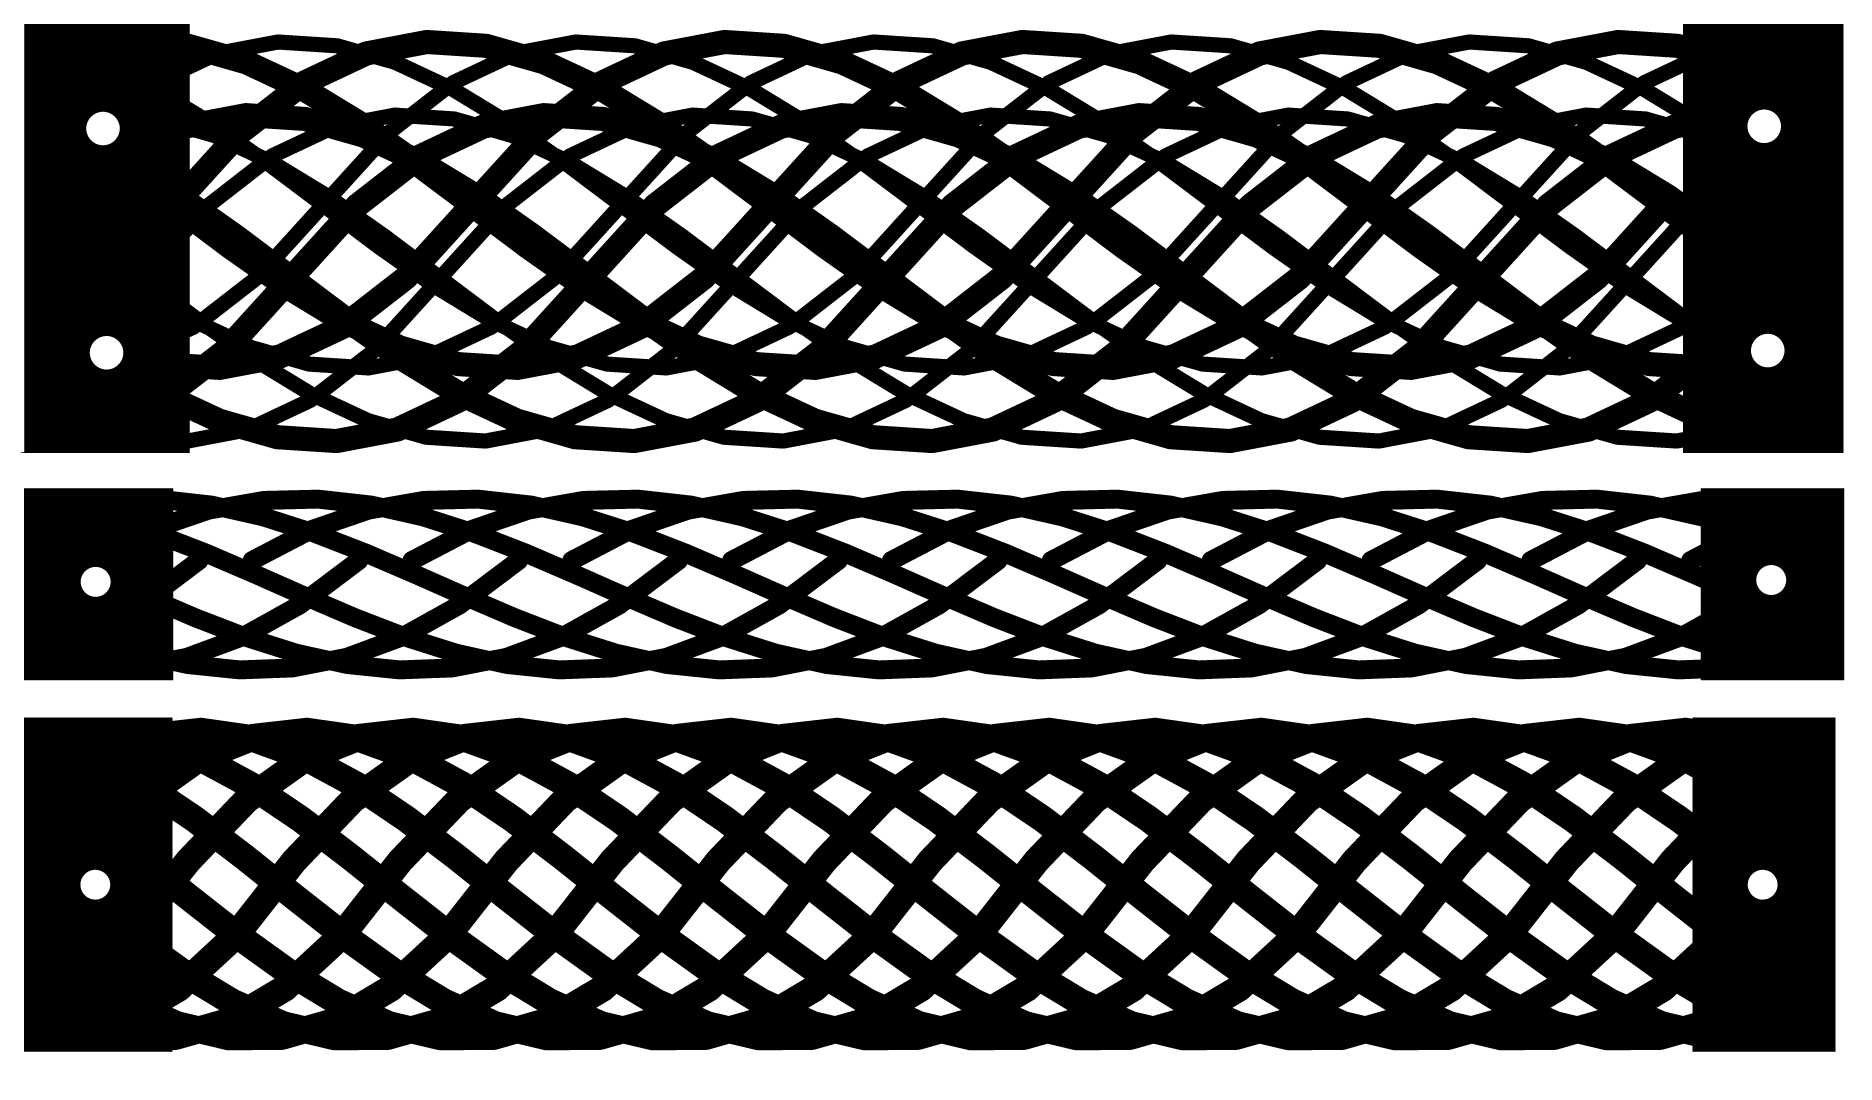
\includegraphics[width=\columnwidth]{images/weave_bracelets.png}
\caption{Alternative bracelet aesthetics}
\label{fig:weave_bracelets}
\end{figure}
\end{center}

\subsection{Personal value in Algorithmic Craft}
Although the aesthetic properties of a finished artifact are important to consider, there are many other components of algorithmic craft that define one's experience.  in all of the workshops, other factors also played an important role in the participant's overall experience. When we asked participants to evaluate their designs, they talked about more than how the object looked. Many participants described the unique quality of their piece:

\begin{quotation}
\textit{``I think it's interesting. I'm assuming this design is unique to me unless someone else goes and makes exactly the same thing, which I highly doubt because of all the random calibration things that I ended up adding."}
\\Youth Participant C
\end{quotation}

\begin{quotation}
Youth Participant C: \textit{``You can�t find it at American eagle. I buy a lot of my bracelets there, and you can�t just go there and find this. I think it�s cool if someone were to say �Oh were did you get that from�, �You can�t find it�. (Laughs). "}
\\Interviewer:\textit{``You can say that you made it yourself, you love how it�s unique?"}
\\YouthParticipant C: \textit{``yeah"}
\end{quotation}

As was the case in the Soft Objects workshops, some of the participants also described how their personal preferences played a strong part in the design of the piece. 

\begin{quotation}
\textit{``usually when you make something you're making it like �oh I hope society likes this� but this[making the bracelet] was about self satisfaction, so I don't have to take into consideration someone else's opinion."}
\\Youth Participant S
\end{quotation}

Comments like these demonstrate participants' awareness of the value in personal craft  practices, in contrast to commercial forms of production. The youth participants entered the workshop with no awareness of the artisanal craft, instead defining craft by its high level of accessibility. By the workshops completion however, the participants described some of the key affordances of craft in their own work, including uniqueness, exclusivity and personal relevancy. Another significant element discussed by participants was their surprise in personally being able to create in this manner through programing. People responded in the following ways when asked to describe their finished piece:
 
\begin{quotation}
 \textit{``II think [the programming] kind of reminded me of learning something difficult in like math, because I don't really like math, but when I figure out something, then I start doing it, and can do it and then I feel proud of myself"}
 \\Youth Participant C
\end{quotation}

 \begin{quotation}
 Interviewer:  \textit{``What stands out to you about your design?"}
 \\Youth Participant S.M.: \textit{``That I actually created it. I'm not really a programing person, doing it and typing it out."}
 \end{quotation}
 
 \begin{quotation}
Youth Participant J: \textit{``It's on computers and I'm terrible at computers and for me to actually get something like this is really big."} 
\\Interviewer:  \textit{``How do you feel about that?"}
\\Youth Participant J:  \textit{``Really proud."}	
\end{quotation}

Finally, participants talked explicitly about the value in being exposed to programing in new ways, and their desire to continue working in computational design and digital fabrication.

 \begin{quotation}
\textit{``I don't know if this is my preferred medium, but I definitely like it.  Making other accessories. If I spent more time playing around with it, I could definitely get something good. 
I'm glad I did it, it's interesting, It's something that I don't have a lot of experience in- just branching out."}
\\Youth Participant R
\end{quotation}

\begin{quotation}
 \textit{``I thought it was a good experience, It was different and it sort of opens your mind to thinking about what else you could do with programing, fashion and stuff like that."}
 \\Youth Participant J
 \end{quotation} 
 
 \begin{quotation}
\textit{``I would love to get into more computational design, I think it's really really cool, because I'm an amateur graphic designer as well."}
\\Youth Participant ST
\end{quotation}

It is apparent that participants not only valued the artifacts they created, but also benefited from the process of producing them. The sense of pride and accomplishment in programing echoes the sentiments of the novice programers in the Soft Objects workshop. The participants in the DressCode workshop were even more vocal about their accomplishment however, in part due to the fact that they were able to program much more independently than in prior workshops. Algorithmic Craft allows people to produce unique objects that have personal and social significance beyond their appearance. Simultaneously, it introduces people to a new context for computation, while simultaneously promoting a sense of personal technological competence. The participants' desire to further engage in similar activities demonstrates the potential for the approach of algorithmic craft to promote continued engagement in programing as a creative practice. 


\subsection{Design history and selection}
\begin{comment}
\begin{quotation}
\textit{``As you can see saved 10 different versions so I would save something, not a completed version of it, but as I was going a long and just do random things to it and see what happened, and if I was physically drawing it, I couldn't just do that unless I wanted to just keep erasing and re-drawing, but in this it's simple as just typing in another number and it will change, but you can always go back to what you had, so it's nice like that."}
\\Youth Participant R
\end{quotation}
\end{comment}



\begin{comment}

beauty
\begin{quotation}
Interviewer: \textit{``Do you think your design is beautiful?"}
\\Youth Participant R: \textit{``No� if it is, it's because of the program, not because something unique I brought to it.. ok I think they're all kind of beautiful- ok I just completely changed my answer. It reminds me of stained glass and I think stained glass is really beautiful."}

social qualities of crafting - maybe for a future direction
role of critique in the process - maybe for a future direction




interest in longer design time, appreciation of needing to learn more
\begin{quotation}
\textit{``Often when I'm doing art and I take a break from it and come back to fresh eyes, then I'll realize that I can do something differently or get something better"}
\\Youth Participant S.M.
\end{quotation}


\end{comment}
\subsection{Relation to Other Design Tools}
\begin{comment}
importance of not starting with blank page

\begin{quotation}
\textit{``I'd rather just have something set and she would just show us how to manipulate the stuff here and it would be easier, instead of showing us all the functions you could do. I would rather have something set for you you, and all I have to do is just plug in numbers."}
\\Youth Participant S.M.
\end{quotation}

\begin{quotation}
\textit{``I've never really done programming like this, but once you have the whole format in and you're just down to changing the numbers then it's fine, but before that if you're not typing something in correctly and you can't find what it is.. but this is relatively simple."}
\\Youth Participant R
\end{quotation}

\begin{quotation}
Interviewer:  \textit{``Would you want to use DressCode again?"}
\\Youth Participant R:\textit{``Sure yeah, now that I feel more comfortable with it and could just start doing it, rather than having to learn. I think it's a good program for someone who's never done anything before...}

\textit{....There's a t-shirt and the symbol on it you can tell was made in here and just attached to the shirt it's not necessarily just making a shirt with the program, but when you combine this with the program you get the shirt, so there's endless possibilities.''}

\end{quotation}


interest in continuing  but comfort in traditional tools
\begin{quotation}
\textit{``I'm more of a sketchup person. I need it directly. I can't program and then play it and then it goes."}
\\Youth Participant S.M.
\end{quotation}

\begin{quotation}
\textit{``They all require some kind of digital design program. We just used DressCode, but what I use is Inkscape or libre office to design my stuff, so it's kind of the same process."}
\\Youth Participant N
\end{quotation}
\end{comment}

\subsection{Prototyping pt 2}
\subsection{Connection to other applications}
\subsection{ challenges in crafting}

